\documentclass[a4paper]{article}
\usepackage[danish]{babel}
\usepackage{amsfonts, amssymb, mathtools, amsthm, amsmath}
\usepackage{graphicx, pgfplots}
\usepackage{url}
\usepackage[dvipsnames]{xcolor}
\usepackage{lastpage}
\usepackage{multicol} 

%loaded last
\usepackage[hidelinks]{hyperref}
\usepackage{bookmark} 

\usepackage{siunitx}
  \sisetup{exponent-product = \cdot,
    output-decimal-marker = {,}}

%Giles Castelles incfig
\usepackage{import}
\usepackage{xifthen}
\usepackage{pdfpages}
\usepackage{transparent}

\newcommand{\incfig}[2][1]{%
  \def\svgwidth{#1\columnwidth}
  \import{./figures/}{#2.pdf_tex}
}

\setlength{\oddsidemargin}{0in}
\setlength{\textwidth}{6.5in}
\setlength{\textheight}{8.8in}
\setlength{\topmargin}{0in}
\setlength{\headheight}{18pt}
\setlength{\parindent}{0pt}
\setlength{\parskip}{0.5\baselineskip}

\usepackage{fancyhdr}
\pagestyle{fancy}

\fancyhead{}
\fancyfoot{}
\fancyfoot[R]{\thepage}
\fancyhead[C]{\leftmark}

\pgfplotsset{compat=newest}

\pgfplotsset{every axis/.append style={
  axis x line=middle,    % put the x axis in the middle
  axis y line=middle,    % put the y axis in the middle
  axis line style={<->,color=black}, % arrows on the axis
}}

\usepackage{thmtools}
\usepackage{tcolorbox}
  \tcbuselibrary{skins, breakable}
  \tcbset{
    space to upper=1em,
    space to lower=1em,
  }

\theoremstyle{definition}

\newtcolorbox[auto counter]{definition}[1][]{%
  breakable,
  colframe=ForestGreen,  %frame color
  colback=ForestGreen!5, %background color
  colbacktitle=ForestGreen!25, %background color for title
  coltitle=ForestGreen!70!black,  %title color
  fonttitle=\bfseries\sffamily, %title font
  left=1em,              %space on left side in box,
  enhanced,              %more options
  frame hidden,          %hide frame
  borderline west={2pt}{0pt}{ForestGreen},  %display left line
  title=Definition \thetcbcounter: #1,
}

\newtcolorbox{greenline}{%
  breakable,
  colframe=ForestGreen,  %frame color
  colback=white,          %remove background color
  left=1em,              %space on left side in box
  enhanced,              %more options
  frame hidden,          %hide frame
  borderline west={2pt}{0pt}{ForestGreen},  %display left line
}

\newtcolorbox[auto counter, number within=section]{eks}[1][]{%
  breakable,
  colframe=NavyBlue,  %frame color
  colback=NavyBlue!5, %background color
  colbacktitle=NavyBlue!25,    %background color for title
  coltitle=NavyBlue!70!black,  %title color
  fonttitle=\bfseries\sffamily, %title font
  left=1em,            %space on left side in box,
  enhanced,            %more options
  frame hidden,        %hide frame
  borderline west={2pt}{0pt}{NavyBlue},  %display left line
  title=Eksempel \thetcbcounter: #1
}

\newtcolorbox{blueline}{%
  breakable,
  colframe=NavyBlue,     %frame color
  colback=white,         %remove background
  left=1em,              %space on left side in box,
  enhanced,              %more options
  frame hidden,          %hide frame
  borderline west={2pt}{0pt}{NavyBlue},  %display left line
}

\newtcolorbox{teo}[1][]{%
  breakable,
  colframe=RawSienna,  %frame color
  colback=RawSienna!5, %background color
  colbacktitle=RawSienna!25,    %background color for title
  coltitle=RawSienna!70!black,  %title color
  fonttitle=\bfseries\sffamily, %title font
  left=1em,              %space on left side in box,
  enhanced,              %more options
  frame hidden,          %hide frame
  borderline west={2pt}{0pt}{RawSienna},  %display left line
  title=Teori: #1,
}

\newtcolorbox[auto counter, number within=section]{sæt}[1][]{%
  breakable,
  colframe=RawSienna,  %frame color
  colback=RawSienna!5, %background color
  colbacktitle=RawSienna!25,    %background color for title
  coltitle=RawSienna!70!black,  %title color
  fonttitle=\bfseries\sffamily, %title font
  left=1em,              %space on left side in box,
  enhanced,              %more options
  frame hidden,          %hide frame
  borderline west={2pt}{0pt}{RawSienna},  %display left line
  title=Sætning \thetcbcounter: #1,
  before lower={\textbf{Bevis:}\par\vspace{0.5em}},
  colbacklower=RawSienna!25,
}

\newtcolorbox{redline}{%
  breakable,
  colframe=RawSienna,  %frame color
  colback=white,       %Remove background color
  left=1em,            %space on left side in box,
  enhanced,            %more options
  frame hidden,        %hide frame
  borderline west={2pt}{0pt}{RawSienna},  %display left line
}

\newtcolorbox{for}[1][]{%
  breakable,
  colframe=NavyBlue,  %frame color
  colback=NavyBlue!5, %background color
  colbacktitle=NavyBlue!25,    %background color for title
  coltitle=NavyBlue!70!black,  %title color
  fonttitle=\bfseries\sffamily, %title font
  left=1em,              %space on left side in box,
  enhanced,              %more options
  frame hidden,          %hide frame
  borderline west={2pt}{0pt}{NavyBlue},  %display left line
  title=Forklaring #1,
}

\newtcolorbox{bem}{%
  breakable,
  colframe=NavyBlue,  %frame color
  colback=NavyBlue!5, %background color
  colbacktitle=NavyBlue!25,    %background color for title
  coltitle=NavyBlue!70!black,  %title color
  fonttitle=\bfseries\sffamily, %title font
  left=1em,              %space on left side in box,
  enhanced,              %more options
  frame hidden,          %hide frame
  borderline west={2pt}{0pt}{NavyBlue},  %display left line
  title=Bemærkning:,
}

\makeatother
\def\@lecture{}%
\newcommand{\lecture}[3]{
  \ifthenelse{\isempty{#3}}{%
    \def\@lecture{Lecture #1}%
  }{%
    \def\@lecture{Lecture #1: #3}%
  }%
  \subsection*{\makebox[\textwidth][l]{\@lecture \hfill \normalfont\small\textsf{#2}}}
}

%Format lim the same way in intext and in display
\let\svlim\lim\def\lim{\svlim\limits}

% horizontal rule
\newcommand\hr{
\noindent\rule[0.5ex]{\linewidth}{0.5pt}
}

\author{Noah Rahbek Bigum Hansen}

\title{Calculus Tau Noter}
\begin{document}
    \maketitle
    % start lectures
    \tableofcontents
    \newpage
    \lecture{1}{26. August 2024}{Differentialregning og stamfunktioner}

Et kritisk punkt er ethvert punkt med en hældning på 0.
\begin{definition} [Definition af kritisk punkt]
  $c$ er et kritisk punkt for $f$ hvis $f'(c) = 0$
\end{definition}


\section{Globale ekstrema (6.1)}
Vi har generelt, at et globalt ekstrema for en funktion kun kan indtræffe i kritiske punkter eller i endepunkter for en funktion. Altså kan alle globale ekstrema findes ved at undersøge alle kritiske punkter og begge (eller det ene eller ingen afhængigt af funktionen) endepunkter kan alle globale ekstrema findes.

\begin{eks} [Maksimum for en funktion]
  Vi ønsker at finde maksimum for funktionen
  \[ 
  f(x) = 3x^{\frac{2}{3}} - 3x^{\frac{5}{3}}
  \]
  på intervallet [0,8].

  For at gøre dette findes den afledte $f'$ som
  \[ 
  f'(x) = 2x^{-\frac{1}{3}} - 5x^{\frac{2}{3}}
  .\]
  Denne sættes dernæst lig 0 som
  \[ 
  f'(x) = 0 = 2x^{-\frac{1}{3}} - 5x^{\frac{2}{3}}
  .\]
  Dernæst kan $x$ isoleres som
  \begin{align*}
    5x^{\frac{2}{3}} &= 2x^{-\frac{1}{3}} \\
    5x &= 2 \\
    x &= \frac{2}{5}
  .\end{align*}
  Altså er funktionens kritiske punkt i intervallet fundet til $x = \frac{2}{5}$. Vi skal altså evaluere funktionen i det kritiske punkt $x = 2 / 5$ og i begge endepunkterne $x = 0$ og $x = 8$. Vi får altså at
  \begin{align*}
    f(0) &= 0 \\
    f(8) &= 12 - 96 = -84 \\
    f(\frac{2}{5}) &= \num{0,977} 
  .\end{align*}
  Altså er det kritiske punkt $x = 2 / 5$ altså et maksimum. 
\end{eks}


\section{Maksimeringsproblemer (6.2)}

\begin{eks} [Maksimeringsproblem i to variable]
  Vi ønsker at finde to positive tal $x$ og $y$ der opfylder
  \[ 
  x + 3y = 30
  \]
  så $x^2y$ bliver maksimeret.
  \bigbreak
  Vi ønsker altså at maksimere
  \[ 
  m(x,y) = x^2y
  \]
  For $x+3y = 30$. Altså findes først et udtryk for $y$ som
  \[ 
  x + 3y = 30 \implies y = 10 - \frac{x}{3}
  .\]
  Dette indsættes i $m(x,y)$ som
  \[ 
  m(x,y) = x^2 \cdot \left( 10 - \frac{x}{3} \right) = 10x^2 - \frac{x^3}{3}
  .\]
  Vi ønsker nu at finde optimeringsgrænserne. Vi ved at $x, y < 0$. Vi har fra før at
  \begin{align*}
    y &> 0 \\
    10 - \frac{x}{3} &> 0 \\
    10 &> \frac{x}{3}
    x &< 30
  .\end{align*}
  Vi har altså, at $0 < x < 30$. Dermed skal $m(x,y)$ maksimeres for $0 < x < 30$. Vi finder de kritiske punkter som
  \begin{align*}
    0 &= m'(x,y) \\
    0 &= 20x - x^2 \\
    0 &= x(20 - x) \\
  .\end{align*}
  Altså er $x = 0$ og $x = 20$ løsninger, dog forkastes $x = 0$ da denne ikke er inde for optimeringsgrænsen. Vi kan dermed evaluere funktionen i begge endepunkter og i det kritiske punkt som
  \begin{align*}
    f(0) &= 0 \\
    f(30) &= 0 \\
    f(20) &= \num{1333,33}\ldots  
  .\end{align*}
  Altså er funktionen maksimeret i $x = 20$. Dette tilsvarer en værdi af $y$ på
  \begin{align*}
    y &= 10 - \frac{20}{3}
    &= \frac{30-20}{3} \\
    &= \frac{10}{3}
  .\end{align*}
\end{eks}

\section{Stamfunktioner og ubestemte integraler (7.1)}
\begin{definition} [Stamfunktion]
  $F(x)$ er en stamfunktion til $f(x)$ hvis der gælder at $F'(x) = f(x)$.
\end{definition}

\begin{definition} [Ubestemt integrale]
  Lad $F(x)$ være en stamfunktion til $f(x)$. Så er det ubestemte integrale af $f(x)$ givet ved
  \[ 
  \int f(x) \, \mathrm{d}x  = F(x) + C
  \]
  Hvor $C$ er en konstant.
\end{definition}

    \newpage
    \section{Simple integraler og differentialer}
\begin{table}[ht]
\begin{tabular}{|c|c|c|}
\hline
$f(x)$             & $f'(x)$                              & $F(x)$                                           \\ \hline
$kx^n$             & $n\cdot k x^{n-1}$                   & $\frac{k}{n+1} x^{n+1} + C$                      \\ \hline
$ke^{cx}$          & $ck \cdot e^{cx}$                    & $\frac{k}{c} \cdot e^{cx} + C$                   \\ \hline
$kx \cdot e^{cx}$  & $(ckx + k)e^{cx}$                    & $\frac{k}{c^2} \cdot \left( cx - 1 \right)e^{cx}$ \\ \hline
$ka^{cx}$          & $ck\cdot \ln(a) \cdot a^{cx}$        & $\frac{ka^{cx}}{c \cdot \ln(a)} + C$             \\ \hline
$\ln(x)$           & $\frac{1}{x}$                        & $x \cdot (\ln(x) - 1) + C$                       \\ \hline
$\log_a(x)$        & $\frac{1}{x \ln(a)}$                 & $\frac{x \cdot (\ln(x)-1)}{\ln(a)} + C$          \\ \hline
$\frac{1}{x}$      & $- \frac{1}{x^2}$                    & $\ln(x) + C$                                     \\ \hline
$\frac{1}{ax+b}$   & $ - \frac{a}{(ax+b)^2}$              & $\frac{ln(ax + b)}{a} + C$                       \\ \hline
$A\sin(kx + \phi)$ & $kA \cdot \cos(kx + \phi)$           & $- \frac{A}{k} \cos(kx + \phi) + C$              \\ \hline
$A\cos(kx+\phi)$   & $-kA \cdot \sin(kx + \phi)$          & $\frac{A}{k} \sin(kx + \phi) + C$                \\ \hline
$A\tan(kx + \phi)$   & $kA \cdot \left( \tan(kx+\phi)^2 + 1 \right)$               & $\frac{-a}{2k} \left( \ln \left( \frac{1}{\tan(kx + \phi)^2 + 1} \right) \right) + C$ \\ \hline
$f(x) + g(x)$      & $f'(x) + g'(x)$                      & $F(x) + G(x) + C$                                \\ \hline
$f(x) \cdot g(x)$  & $f(x)g'(x) + f'(x)g(x)$              & $f(x)G(x) - \int f'(x)G(x) \, \mathrm{d}x + C$   \\ \hline
$f(g(x))$          & $g'(x) f'(g(x))$                     & Brug substitution                                \\ \hline
$\frac{f(x)}{g(x)}$  & $\frac{g(x)f'(x) - f(x) g'(x)}{\left(g(x) \right)^2}$       & Brug delvis integration                                                               \\ \hline
$\frac{f'(x)}{f(x)}$ & $\frac{f''(x)}{f(x)} - \left( \frac{f'(x)}{f(x)} \right)^2$ & $\ln \left| g(x) \right| + C$                                                         \\ \hline
$\sqrt[b] x^a$     & $\frac{a}{b}\cdot x^{\frac{a}{b}-1}$ & $\frac{x^{a / b + 1}}{a / b + 1}  + C$           \\ \hline
\end{tabular}
\end{table}

\section{Komplicerede integraler og differentialer}
Hvis dit udtryk er på formen
\[ 
\int f \left( g(x) \right) \cdot g'(x) \, \mathrm{d}x 
\]
Brug da \underline{\hyperref[afs:intsub]{Integration ved Substitution}}. Hvis dit udtryk er på formen
\[
  \int f(x) g'(x) \, \mathrm{d}x 
.\]
Brug da \underline{\hyperref[afs:delint]{Delvis Integration}}. Hvis dit udtryk er på formen
\[ 
\frac{\mathrm{d}}{\mathrm{d}x} f(g(x))
.\]
Brug da \underline{\hyperref[afs:aflkæd]{Kædereglen}}.

\subsection{Kædereglen} \label{afs:aflkæd}
Kædereglen foreskriver at den afledte
\[ 
\frac{\mathrm{d}}{\mathrm{d}x} f \left( g(x) \right) = f' \left( g(x) \right) \cdot g'(x)
\]

    \newpage
    \lecture{2}{2. September 2024}{Integration}

\section{Integration ved substitution (7.2)} \label{afs:intsub}
Integration ved substitution kan forstås som kædereglens inverse. 
\begin{definition} [Integration ved substitution]
  Lad $f$ og $g$ være funktioner. Med substitutionen $u = g(x)$ er
  \[ 
  \int f(g(x))g'(x)\, \mathrm{d}x = \int f(u) \, \mathrm{d}u = F(u) = F(g(x))
  \]
  hvor $F$ er en stamfunktion til $f$. Ofte skrives
  \[ 
  \mathrm{d}u = g'(x) \, \mathrm{d}x 
  .\]
  Hvilket gør det lettere at huske formlen.
\end{definition}

\begin{eks} [Et simpelt eksempel]
  Vi ønsker at bestemme
  \[ 
  \int 8x \left( 4x^2 + 8 \right)^{6} \, \mathrm{d}x
  .\]
  Vi sætter $u = 4x^2 + 8$ og får dermed $\mathrm{d}u = 8x \, \mathrm{d}x$. Dermed fås
  \[ 
  \int u^{6} \, \mathrm{d}u = \frac{u^{7}}{7}
  .\]
  Sættes definitionen af $u$ ind i det ovenstående fås
  \[ 
  \int 8x \left( 4x^2 + 8 \right)^{6} = \frac{u^{7}}{7} = \frac{\left( 4x^2 + 8 \right)^{7}}{6}
  .\]
\end{eks}

\begin{eks} [Et mere kompliceret eksempel]
  Vi ønsker at finde
  \[ 
  \int x^3 \sqrt{3x^{4} + 10} \, \mathrm{d}x 
  .\]
  Vi sætter $u = 3x^{4} + 10$ og får dermed $\mathrm{d}u = 12x^3$. Ved at gange integralet fra før med $1 = \frac{12}{12}$ bliver integralet til
  \[ 
  \frac{1}{12}\int \sqrt{3x^{4} + 10} 12x^3 \, \mathrm{d}x
  .\]
  Dernæst kan $u$ indsættes som
  \[ 
  \frac{1}{12} \int \sqrt{u} \, \mathrm{d}u = \frac{1}{12} \left( \frac{2}{3} u^{\frac{3}{2}} \right) = \frac{1}{18} u^{\frac{3}{2}}
  .\]
  Definitionen af $u$ kan nu indsættes igen som
  \[ 
  \int x^3 \sqrt{3x^{4} + 10} \, \mathrm{d}x = \frac{1}{18} \left( 3x^{4} + 10 \right)^{\frac{3}{2}}
  .\]
\end{eks}

\section{Fundamentalsætningen for calculus (7.4)}

\begin{definition} [Bestemte integraler]
  Hvis $f$ er en positiv funktion så angiver det bestemte integral 
  \[ 
  \int_{a}^{b} f(x) \, \mathrm{d}x 
  \]
  arealet mellem $x$-aksen og funktionen $f$ over intervallet $[a,b]$.
\end{definition}

\begin{sæt} [Fundmentalsætningen for calculus]
  Hvis $f$ er en kontinuert funktion på intervallet $[a,b]$, og $F$ er en stamfunktion til $f$ så er
  \[ 
  \int_{a}^{b} f(x) \, \mathrm{d}x = F(b) - F(a) = F(x) \bigg|_a^{b}
  .\]
\end{sæt}

\begin{eks} [Simpelt bestemt integral]
  Vi ønsker at finde $\int_{1}^{3} 3x^2 \, \mathrm{d}x$.
  \bigbreak
  Først bestemmes det ubestemte integral som
  \[ 
  \int 3x^2 \, \mathrm{d}x = x^3
  .\]
  Dernæst benyttes fundamentalsætningen for calculus som
  \[ 
  \int_{1}^{3} 3x^2 \, \mathrm{d}x = 3^3 - 1^3 = 26
  .\]
\end{eks}

\begin{eks} [Et mere bøvlet bestemt integral]
  Vi ønsker at finde $\int_{0}^{4} 2x \sqrt{16 - x^2}\, \mathrm{d}x $.
  \bigbreak
  Først findes det ubestemte integral ved at sætte $u = 16 - x^2$ og dermed får $\mathrm{d}u = -2x \, \mathrm{d}x$. Vi kan altså skrive integralet som
  \[ 
  \int 2x \sqrt{16-x^2} \, \mathrm{d}x = -\int \sqrt{u} \mathrm{d}u = -\int u^{\frac{1}{2}} \mathrm{d}u
  .\]
  Dette integral løses nu som normalt som
  \[ 
  -\int u^{\frac{1}{2}} \mathrm{d}u = -\frac{2}{3} u^{\frac{3}{2}} + c
  .\]
  Dermed kan substitutionen sættes tilbage ind som
  \[ 
  -\frac{2}{3} \left( 16-x^2 \right)^{\frac{3}{2}} + c
  .\]
  Og slutteligt kan integrationsgrænserne igen indsættes som
  \begin{align*}
  \int_{0}^{4} 2x \sqrt{16-x^2} \, \mathrm{d}x &= -\frac{2}{3} \left( 16-x^2 \right)^{\frac{3}{2}} \bigg|_0^{4} \\
  &= -\frac{2}{3} \left( \left( 16-4^2 \right)^{\frac{3}{2}} - \left( 16-0^2 \right)^{\frac{3}{2}} \right) \\
  &= -\frac{2}{3}\left( 0^{\frac{3}{2}} - 16^{\frac{3}{2}} \right) \\
  &= \frac{2}{3} \cdot 16^{\frac{3}{2}} \\
  &= \frac{2}{3} \cdot 16 \cdot \sqrt{16} \\
  &= \frac{128}{3}
  .\end{align*}
\end{eks}
\textit{Note fra Basse:} Hvis man laver en fortegnsfejl til eksamen er det vigtigt at man laver en mere -- så passer pengene. Man skal altid have et lige antal fortegnsfejl.

\section{Delvis integration (8.1)}
Delvis integration er produktreglens pendant på samme måde som integration ved substitution er kædereglens pendant.
\begin{sæt} [Delvis integration] \label{afs:delint}
  Der gælder
  \[
    \int u(x)v'(x) = u(x)v(x) - \int u'(x)v(x) \, \mathrm{d}x
  .\]
  Med $\mathrm{d}u = u'(x) \, \mathrm{d}x$ og $\mathrm{d}v = v'(x) \, \mathrm{d}x$ kan det ovenstående skrives som
  \[ 
  \int u \mathrm{d}v = uv - \int v \mathrm{d}u
  .\]
\end{sæt}

\begin{eks} [Simpelt integral med delvis integration]
  Vi ønsker at bestemme
  \[ 
  \int x e^{-2x} \, \mathrm{d}x
  .\]
  \bigbreak
  Vi sætter $u = x$ og $\mathrm{d}v = e^{-2x}$. Vi ønsker at finde et udtryk for $v$ og derfor integreres $\mathrm{d}v = e^{-2x}$ som
  \[ 
  \int e^{-2x} \, \mathrm{d}x = -\frac{1}{2}e^{-2x}
  .\]
  Vi får dermed
  \[ 
  \int x e^{-2x} = x \cdot -\frac{1}{2}e^{-2x} - \int -\frac{1}{2} e^{-2x} \, \mathrm{d}x = -\frac{1}{2}x e^{-2x} + \frac{1}{2} \int e^{-2x} \, \mathrm{d}x
  .\]
  Vi har tidligere fundet $\int e^{-2x} \, \mathrm{d}x  = -\frac{1}{2}e^{-2x}$. Dermed bliver det ovenstående
  \begin{align*}
  \int x e^{-2x} \, \mathrm{d}x &= -\frac{1}{2}x e^{-2x} + \frac{1}{2} \cdot \left( -\frac{1}{2}e^{-2x} \right) \\
  &= -\frac{1}{2}x e^{-2x} - \frac{1}{4}e^{-2x}
  .\end{align*} 
\end{eks}

\begin{eks} [Et mere kompliceret eksempel med delvis integration]
  Vi ønsker at finde
  \[ 
  \int \ln 2x \, \mathrm{d}x
  .\]
  \bigbreak
  Vi sætter $u = \ln 2x$ og dermed fås $\mathrm{d}u = \frac{1}{2x} \cdot 2 \, \mathrm{d}x = x \, \mathrm{d} \frac{1}{x} $ dermed fås $\mathrm{d}v = \mathrm{d}x$. Dermed bliver det ovenstående til
  \begin{align*}
  \int \ln 2x \, \mathrm{d}x &= \ln (2x) \cdot x - \int x \cdot \frac{1}{x} \, \mathrm{d}x  \\
  &= \ln (2x) \cdot x - x \\
  &= x \left( \ln (2x) - 1 \right)
  .\end{align*}  
\end{eks}

\begin{eks} [Dobbelt delvis integation]
  Vi ønsker at finde
  \[ 
  \int x^2 e^{x} \, \mathrm{d}x 
  .\]
  \bigbreak
  Vi sætter $u = x^2$ og $\mathrm{d}v = e^{x}$. Dermed fås $\mathrm{d}u = 2x$ og $v = e^{x}$. Det ovenstående integral bliver derfor
  \[
  \int x^2 e^{x} \, \mathrm{d}x = x^2 e^{x} - 2\int x  e^{x} \, \mathrm{d}x
  .\]
  Vi kan dernæst løse $\int x e^{x} \, \mathrm{d}x$ med delvis integration ved at sætte $u = x$, $\mathrm{d}u = \mathrm{d}x$, $\mathrm{d}v = e^{x} \, \mathrm{d}x $ og dermed $v = e^{x}$. Vi får dermed
  \[
    \int x e^{x} \, \mathrm{d}x = x e^{x} - \int e^{x} \, \mathrm{d}x = x e^{x} - e^{x} = e^{x} \left( x - 1 \right)
  .\]
  Dette kan sættes tilbage ind i det første integral som
  \[ 
  x^2 e^{x} - 2 \int x e^{x} \, \mathrm{d}x = x^2 e^{x} - 2 e^{x} \left( x-1 \right) = e^{x} \left( x^2 - 2(x-1) \right)
  .\]
\end{eks}

\begin{eks} [Et hurtigt integral med delvis integration]
  Hvis vi ønsker at finde
  \[ 
  \int \sin(x) e^{x} \, \mathrm{d}x 
  \]
  kan vi sætte $u = \sin x$ og dermed få $\mathrm{d}u = \cos x$. Dette virker umiddelbart ikke til at give et nemmere integral men hvis formlen bruges igen fås $\mathrm{d\,d}u = -\sin(x)$ og vha. delvis integration fås dermed et udtryk hvor det samme integral står på begge sider af lighedstegnet og løsningen til dette integral kan derfor isoleres herfra. Dermed kan integralet løses uden egentligt at beregne et integral. Dette er vist nedenfor
  \begin{align*}
    \int \sin x e^{x}\, \mathrm{d}x &= \sin x e^{x} - \int \cos x e^{x} \, \mathrm{d}x \\
    \int \cos x e^{x} \, \mathrm{d}x &= \cos x e^{x} - \int - \sin x e^{x} \, \mathrm{d}x \\
    \int \sin x e^{x} \, \mathrm{d}x &= \sin x e^{x} - \cos x e^{x} - \int \sin x e^{x} \, \mathrm{d}x  \\
    2 \int \sin xe^{x} \, \mathrm{d}x &= \sin x e^{x} - \cos x e^{x} \\
    \int \sin xe^{x} \, \mathrm{d}x &= \frac{\sin x e^{x} - \cos x e^{x}}{2}
  .\end{align*}
\end{eks}

\section{Uegentlige integraler}
Et uegentligt integral er ethvert integral, der har enten $\infty$, $-\infty$ eller begge som en af eller begge sine integrationsgrænser.
\begin{sæt} [Uegentlige integraler]
  For et integral med øvre integrationsgrænse på $\infty$ har vi
  \[ 
  \int_{a}^{\infty} f(x) \, \mathrm{d}x = \lim_{b \to \infty } \int_{a}^{b} f(x) \, \mathrm{d}x
  .\]
  Og tilsvarende for et integral med nedre integrationsgrænse på $-\infty$ har vi
  \[ 
  \int_{-\infty}^{b} f(x) \, \mathrm{d}x = \lim_{a\to -\infty} \int_{a}^{b} f(x) \, \mathrm{d}x 
  .\]
  For et integral med funktionsgrænser på $-\infty$ og $\infty$ har vi i stedet
  \[ 
  \int_{-\infty}^{\infty} f(x) \, \mathrm{d}x = \int_{-\infty}^{0} f(x) \, \mathrm{d}x + \int_{0}^{\infty} f(x) \, \mathrm{d}x 
  .\]
\end{sæt}

\begin{eks} [Eksempel på beregning af et uegentligt integral]
  Vi ønsker at finde
  \[ 
  \int_{1}^{\infty} x^{-\frac{3}{2}} 
  .\]
  \bigbreak
  Først benyttes sætningen fra ovenfor så vi får at
  \[ 
    \int_{1}^{\infty} x^{-\frac{3}{2}} \, \mathrm{d}x = \lim_{b \to \infty} \int_{1}^{b} x^{-\frac{3}{2}}\, \mathrm{d}x 
  .\]
  Vi bestemmer dernæst integralet som
  \[ 
  \int_{1}^{\infty } x^{-\frac{3}{2}} \, \mathrm{d}x = -2 x^{-\frac{1}{2}} \bigg|_{1}^{\infty} = -2 \left( \frac{1}{\sqrt{b}} - 1 \right) = 2 \left( 1 - \frac{1}{\sqrt{b}}\right)
  .\]
  Vi lader derefter $b \to \infty$ vi får dermed
  \[
  \lim_{b \to \infty} \sqrt{b} = \infty
  .\]
  Vi får dermed
  \begin{align*}
  \int_{1}^{\infty} x^{-\frac{3}{2}} \, \mathrm{d}x &= 2 \left( 1 - \frac{1}{\infty } \right) \\
  &= 2 \cdot 1 \\
  &= 2
  .\end{align*}
  Dermed er løsningen fundet.
\end{eks}

    \newpage
    \lecture{3}{9. November 2024}{Komplekse tal}

\section{Kort gennemgang af trionometri}
For vektorer i planen gælder, at
\[ 
u\cdot v = |u||v|\cos\theta
\]
hvor $\theta$ er vinklen mellem de to vektorer og $\cdot$ angiver det indre produkt, også kendt som prikproduktet.

\textit{Note:} Der er ingen lyd på optagelsen herfra og de næste 40 minutter frem så de næste par noter er taget alene på baggrund af en meget lille video, derfor tages der forbehold for fejl i det følgende, omend dette heller ikke er den vigtigste del af forelæsningen.

\subsection{Additionsformlen for cosinus}
Givet en vinkel $\theta = \alpha + \beta$ kan $\cos\theta$ findes vha. en additionsformel såfremt $\cos\alpha$ og $\cos\beta$ er kendt. Vi kan opskrive prikproduktet som
\begin{align*}
\cos (\beta - \alpha) &= \Vec{u}\cdot \Vec{v} \\
&= \begin{pmatrix}
  \cos \beta \\
  \sin \beta
\end{pmatrix}
\cdot
\begin{pmatrix}
  \cos\alpha \\
  \cos\beta
\end{pmatrix} \\
&= \cos\alpha \cos\beta + \sin\alpha \sin\beta
.\end{align*}
Vi har altså nu vist at
\[ 
  \cos(\beta-\alpha) = \cos\alpha \cos\beta + \sin\alpha \sin\beta \implies \cos(\alpha + \beta) = \cos{(-\alpha)}\cos\beta + \sin{(-\alpha)}\sin\beta
.\]
Idet $\cos\alpha = \cos(-\alpha)$ og $\sin(-\alpha) = -\sin\alpha$ kan det ovenstående omskrives til
\[ 
\cos(\alpha + \beta) = \cos\alpha \cos\beta - \sin\alpha \sin\beta
.\]

\subsection{Additionsformlen for sinus}
Idet $\cos$ og $\sin$ blot er faseforskydninger af hinanden må følgende udtryk for $\sin(\alpha + \beta)$ gælde
\[ 
\sin(\alpha + \beta) = -\cos(\alpha + \beta + \frac{\pi}{2})
.\]
Vi kan da benytte additionsformlen for $\cos$ på det ovenstående som
\[ 
\sin(\alpha + \beta) = -\left( \cos\alpha \cos(\beta + \frac{\pi}{2}) \right) - \sin\alpha \sin(\beta + \frac{\pi}{2})
.\]
Vi har at $\cos(\beta + \frac{\pi}{2}) = -\sin\beta$ og $\sin(\beta + \frac{\pi}{2}) = \cos\beta$ derfor kan det ovenstående omskrives til
\[ 
\sin(\alpha + \beta) = \cos\alpha \sin\beta + \sin\alpha \cos\beta
.\]

\section{Introduktion til komplekse tal}
\begin{definition} [Den imaginære enhed]
  Den imaginære enhed $i$ opfylder
  \[ 
  i^2 = -1
  .\]
\end{definition}

\begin{definition} [Komplekse tal]
  Et komplekst tal $z \in \mathbb{C}$ er givet ved
  \[ 
  z = a + ib
  \]
  hvor $a \in \mathbb{R}$ og $b \in \mathbb{R}$. Det ovenstående kaldes også \textit{standardformen} for et komplekst tal.
\end{definition}

\begin{definition} [Realdelen og imaginærdelen af et komplekst tal]
  Realdelen af det komplekse tal $z = a + ib$ $\Re(z)$ er givet som
  \[ 
    \Re( z ) = a
  .\]
  Tilsvarende er imaginærdelen af $z$ $\Im(z)$ givet ved
  \[ 
    \Im( z ) = b
  .\]
\end{definition}

\subsection{Regneregler for komplekse tal}
Lad $z_1 = a_1 + ib_1$ og $z_2 = a_2 + ib_2$ da gælder følgende relationer
\begin{align*}
  z_1 + z_2 &= a_1 + a_2 + i(b_1 + b_2) \\
  z_1z_2 &= (a_1 + ib_1)(a_2 + ib_2) = a_1a_2 - b_1b_2 + i(a_1b_2 + a_2b_1)
.\end{align*}

\begin{eks} [Multiplikation af to komplekse tal]
  Vi ønsker at løse
  \[ 
    (3+2i)(4-2i)
  .\]
  Vi ganger parenteserne ud og får
  \begin{align*}
    (3+2i)(4-2i) &= 3\cdot 4 + 2i(-2i) + 3(-2i) + 2i \cdot 4 \\
    &= 12 + (-4)i^2 + -6i + 8i\\
    &= 16 + 2i
  .\end{align*}
\end{eks}

\subsection{Det komplekse talplan}
Det komplekse talplan er et $(\Re, \Im)$-plan således at den traditionelle $x$-akse angiver realdelen af det komplekse tal og den traditionelle $y$-akse angiver imaginærdelen af det komplekse tal. Ethvert komplekst tal vil da kunne angives som et punkt på dette plan, mens ethvert reelt tal vil kunne findes langs $\Re$-aksen (``$x$''-aksen).

\begin{definition} [Absolut værdi]
  Den absolutte værdi $|z|$ af et komplekst tal $z = a + ib$ er givet som
  \[ 
  |z| = \sqrt{a^2 + b^2}
  .\]
  Dette tilsvarer afstanden fra det komplekse tal til origo i det komplekse talplan.
\end{definition}

\begin{definition} [Kompleks konjugering]
  Den komplekse konjugering $\overline{z}$ af det komplekse tal $z = a + ib$ er
  \[ 
  \overline{z} = a -ib
  .\]
  Altså er den komplekse konjugering et fortegnsskifte på imaginærdelen $\Im(z)$.
\end{definition}

Desuden gælder det at for to komplekse tal $z_1$ og $z_2$ er $|z_1 + z_2|$ afstanden mellem $z_1$ og $z_2$ i det komplekse talplan.

\begin{eks} [Afstande i det komplekse talplan]
  Vi ønsker at bestemme hvilke af de komplekse tal
  \begin{align*}
  z_1 &= 4 + 2i \\
  z_2 &= 3-3i \\
  z_3 &= -1
  \end{align*}
  der ligger tættest på hinanden i det komplekse talplan.
  \bigbreak
  Først findes afstandende mellem alle tre tal i det komplekse talplan som
  \begin{align*}
    |z_1 - z_2| &= |4-3 + 2i + 3i| = |1 - 5i| = \sqrt{26} \\
    |z_1 - z_3| &= |4 + 1 + 2i| = |5 + 2i| = \sqrt{29} \\
    |z_2 - z_3| &= |3 + 1 - 3i| = |4 - 3i| = \sqrt{25} = 5
  .\end{align*}
  Altså er de to tal der ligger tættest på hinanden i det komplekse talplan ud af de givne tal $z_2$ og $z_3$
\end{eks}

\subsection{Division med komplekse tal}
En vigtig udregning er at
\[ 
z \overline{z} = (a+ib)(a-ib) = a^2 + b^2 = |z|^2
.\]
Altså giver produktet af et komplekst tal og dens konjugerede et reelt tal. Dette er et yderst vigtigt resultat. Hvis der divideres med $|z|^2$ på begge sider får vi nemlig at
\[ 
z \frac{\overline{z}}{|z|^2} = 1 \implies \frac{1}{z} = \frac{\overline{z}}{|z|^2}
.\]
Altså har vi fundet $z$'s multiplikative inverse til $\frac{\overline{z}}{|z|^2}$. Dette gør det da muligt at dividere da
\[ 
\frac{z_1}{z_2} = z_1 \frac{1}{z_2} = z_1 \frac{\overline{z_2}}{|z_2|^2}
.\]

\subsection{Samling af nyttige regneregler for komplekse tal}
Vi har generelt følgende regneregler for komplekse tal ($z_1 = a_1 + ib_1, z_2 = a_2 ib_2$)
\begin{align*}
  z_1 + z_2 &= a_1 + a_2 + i(b_1 + b_2) \\
  z_1 - z_2 &= a_1 - a_2 + i(b_1 - b_2) \\
  z_1z_2 &=  a_1a_2 - b_1b_2 + i(a_1b_2 + a_2b_1) \\
  \frac{z_1}{z_2} &= \frac{z_1 \overline{z_2}}{|z_2|^2} \\
  |\overline{z}| &= |z| \\
  |z_1z_2| &= |z_1||z_2| \\
  \left| \frac{z_1}{z_2} \right| &= \frac{|z_1|}{|z_2|} \\
  \overline{z_1z_2} &= \overline{z_1} \overline{z_2} \\
  \overline{\left( \frac{z_1}{z_2} \right)} &= \frac{\overline{z_1}}{\overline{z_2}}
.\end{align*}

\begin{eks} [Eksempel på division]
  Vi ønsker at finde
  \[ 
  \frac{1 +2i}{2-3i}
  .\]
  \bigbreak
  Vi får vha. regnereglen at
  \begin{align*}
    \frac{1+2i}{2-3i} &= \frac{(1+2i)(2+3i)}{|2+3i|^2} \\
    &= \frac{2 - 6 + 3i + 4i}{4^2 + 3^2} \\
    &= \frac{-4}{13} \frac{7}{13}i
  .\end{align*}
\end{eks}

\begin{eks} [Eksempel på brug af flere regneregler med division]
  Vi ønsker at finde
  \[ 
  \left| \frac{4i \overline{(3+4i)}}{(1+2i)(1-i)} \right|
  .\]
  Vi benytter regnereglerne som
  \begin{align*}
  \left| \frac{4i \overline{(3+4i)}}{(1+2i)(1-i)} \right| &= \frac{|4i| |3+4i|}{|1+2i||1-i|} \\
  &= \frac{4 \sqrt{25}}{\sqrt{5}\sqrt{2}} \\
  &= \frac{20}{\sqrt{10}} \\
  &= 2 \sqrt{10}
  .\end{align*}
\end{eks}

\section{Polær form af komplekse tal}
For et komplekst tal $z$ i det komplekse talplan kan et linjestykke fra origo til det komplekse tal tegnes. Vinklen $\theta$ mellem dette linjestykke og $\Re$-aksen betegnes et \textit{argument} af $x$. Vi kan opskrive følgende udtryk for $z$ som
\[ 
\begin{pmatrix}
  a \\
  b
\end{pmatrix}
=
\begin{pmatrix}
  |z| \cos\theta \\
  |z| \sin\theta
\end{pmatrix}
=
|z|(\cos\theta + i \sin\theta)
.\]

\begin{definition} [Den komplekse eksponentialfunktion]
  Den komplekse eksponentialfunktion $e^{i\theta}$ er defineret som
  \[ 
  e^{i\theta} = \cos\theta + i \sin\theta
  .\]
  Altså kan et komplekst tal $z$ skrives på polær form som
  \[ 
  z = |z|e^{i \theta}
  .\]
\end{definition}

\subsection{Multiplikation på polær form}
For $z_1 = r_1 e^{i\theta_1}$ og $z_2 = r_2 e^{i\theta_2}$ gælder:
\begin{align*}
  z_1z_2 &= r_1r_2(\cos\theta_1 + i \sin\theta_1)(\cos\theta_2 + i \sin\theta_2) \\
  &= r_1r_2 \left( \left( \cos\theta_1 \cos\theta_2 - \sin\theta_1 \sin\theta_2 \right) + i \left( \cos\theta_1 \sin\theta_2 + \sin\theta_1 \cos\theta_2 \right) \right) \\
  &= r_1r_2 \left( \cos(\theta_1 + \theta_2) + i \sin(\theta_1 + \theta_2)\right) \\
  &= r_1r_2 e^{i(\theta_1 + \theta_2)}
.\end{align*}
Bemærk at ovenstående medfører at
\[ 
z^{n} = r^{n}e^{i n\theta}
.\]

\begin{eks} [Omregning fra standard til polær form]
  Vi ønsker at skrive $z = -2 + 2i$ på polær form.
  \bigbreak
  Først indses at absolutværdien af $z$ er
  \[ 
  |z| = \sqrt{2^2 + 2^2} = \sqrt{8}
  .\]
  Det indses at vinklen $\theta$ er i 2. kvadrant og derfor må $\theta$ være lig $\frac{\pi}{2}$ plus lidt mere. Herfra kan vi benytte trigonometri således at vi får en retvinklet trekant med kateter med længde 2 og hypotenuse med længde $\sqrt{8}$. For at finde vinklen kan trigonometri benyttes som
  \[ 
    \cos^{-1}(\frac{2}{\sqrt{2}}) = \cos^{-1}(\frac{\sqrt{2}}{2}) = \frac{\pi}{4}
  .\]
  Altså er den samlede vinkel $\theta$
  \[ 
  \theta = \frac{\pi}{2} + \frac{\pi}{4} = \frac{3\pi}{4}
  .\]
\end{eks}

\subsection{Kvadratrødder af komplekst tal}
Givet et komplekst tal $d = re^{i\theta}$ er dets kvadratødder
\[ 
  \pm \sqrt{d} = \pm \sqrt{r}e^{i \frac{\theta}{2}}
.\]
Bemærk, at ethvert komplekst tal ha præcis to kvadradtrødder.

\subsection{Andengradsligning}
For $a, b, c \in \mathbb{C}$ og med $a \neq 0$ er en general andengradsligning
\[ 
a z^2 + bz + c = 0
\]
er kvadratroden af diskriminanten $D$ givet ved
\[ 
\pm \sqrt{D} = 2a z + b
.\]
Og andengradsligningens generelle løsning er 
\[ 
z = \frac{-b \pm \sqrt{D}}{2a}
.\]

Vi har følgende fremgangsmåde for at løse en andengradsligning $a z^2 + bz + c = 0$:
\begin{enumerate}
  \item Udregn diskriminanten $D = b^2 - 4ac$
  \item Bestem polær form $D = re^{i\theta}$
  \item Bestem kvadratrødderne $\pm \sqrt{D} = \pm \sqrt{r}e^{i \frac{\theta}{2}}$
  \item Indsæt i formlen for løsning af andengradsligning:
\end{enumerate}
    \[ 
    z = \frac{-b \pm\sqrt{D}}{2a}
    .\]

    \newpage
    \lecture{4}{16. September 2024}{Talfølger og uendelige rækker}

\section{Talfølger}
En talfølge er typisk defineret enten
\begin{itemize}
  \item ved en lukket formel
  \item eller induktivt
\end{itemize}

\begin{eks} [Eksempel på induktivt defineret talfølge]
  Givet en initialværdi $a_1 = A$ og et induktionstrin
  \[ 
  a_{n+1} = \frac{1}{2}\left( a_n + \frac{A}{a_n+1} \right)
  \]
  er en induktivt defineret talfølge givet. Det viser sig faktisk at den ovenstående talfølge netop bliver $\sqrt{A}$ for $n \to \infty$.
\end{eks}

\subsection{Fibonaccis talfølge}
Et andet berømt eksempel på en induktivt defineret talfølge er Fibonaccis talfølge der er givet ved initialværdierne $a_0 = 0, a_1 = 1$ og induktionstrinnet
\[ 
a_n = a_{n-1} + a_{n-2}
.\]
Det viser sig at Fibonaccis talfølge faktisk kan skrives på en lukket form som
\[ 
a_n = \frac{1}{\sqrt{5}} \left( \left( \frac{1 + \sqrt{5}}{2} \right)^{n} - \left( \frac{1 - \sqrt{5}}{2} \right)^{n} \right)
.\]
Her kan det bemærkes at $\frac{1 + \sqrt{5}}{2}$ er det gyldne snit.

\section{Konvergens/divergens af talfølger} \label{afs:konv}
\begin{definition} [Konvergens af talfølger]
  En talfølge ${a_n}_{n = 1}^{\infty} = a_1, a_2, a_3,\ldots$ kaldes \textit{konvergent} med \textit{grænseværdi} $a$, skrevet
  \[ 
  a_n \to a \quad \text{for} \quad n\to \infty \qquad \text{eller} \qquad \lim_{n \to \infty } a_n = a
  ,\]
  hvis vi for enhver tolerance $\epsilon > 0$ kan gå langt nok ud i talfølgen (fra og med et indeks $N$) så
  \[ 
  n \geq N \implies |a_n - a| < \epsilon
  .\]
  Hvis $n \geq N$ ikke medfører $|a_n - a| <\epsilon$ så kaldes talfølgen ${a_n}_{n = 1}^{\infty}$ i stedet divergent og tilskrives ikke en grænseværdi.
\end{definition}

\begin{eks} [Konvergens af den harmoniske talfølge]
  Vi ønsker at finde ud af om $\frac{1}{n}$ er konvergent mod 0. \bigbreak
  Vi benytter definitionen fra ovenfor som
  \[ 
  |a_n - 0| = \frac{1}{n}
  \]
  så for en tolerance $\epsilon > 0$ gælder
  \[ 
  \frac{1}{n} = |a_n - 0| \leq \epsilon \iff n \geq \frac{1}{\epsilon}
  .\]
  Dermed er det vist, at fra og med et indeks $N \geq \frac{1}{\epsilon}$, så er $a_n$ indenfor en tolerance $\epsilon$ fra 0.
\end{eks}

\begin{eks} [Divergens af simpel alternerende talfølger]
  Vi betragter nu talfølgen givet ved $a_n = (-1)^{n}$
  \[ 
    {a_n}_{n = 1}^{\infty} = -1, 1, -1, 1, \ldots 
  .\]
  Det indses hurtigt at rækken er divergent, da vi aldrig kan vælge en værdi for grænseværdien $a$ således at en tolerance $0 < \epsilon < 2$ er opfyldt.
\end{eks}



\section{Regneregler for grænseværdier}
\begin{sæt} [Regneregler for grænseværdier]
  Lad $\lim_{n \to \infty} a_n = a$ og $\lim_{n \to \infty} b_n = b$, så gælder
  \begin{align*}
  &\lim_{n \to \infty} (a_n + b_n) = a+b \\
  &\lim_{n \to \infty} a_{n} b_{n} = ab \\
  &\lim_{n \to \infty} \frac{a_n}{b_n} = \frac{a}{b} \text{ hvis } b \neq 0 \\
  &\lim_{n \to \infty} f(a_{n}) = f(a) \text{ hvis $f$ er kontinuert i punktet $a$}
  .\end{align*}
\end{sæt}

\begin{eks} [Eksempel på brug af regnereglerne]
  Givet 
  \[ 
  a_n = \frac{17n^{4} + 3n^2 - 5 \cos \left( \frac{1}{n} \right)}{-5n^{4} - 3n^3 e^{\sin \left( \frac{2}{n} \right)}}
  \]
  ønsker vi at bestemme om ${a_n}_{n = 1}^{\infty}$ er konvergent og i så fald hvad dens grænseværdi er.
  \bigbreak
  Vi starter med at forkorte hele udtrykket med $n^{4}$ så vi får
  \[ 
  a_n = \frac{17 + \frac{3}{n^2} - \frac{5}{n^{4}} \cos \left( \frac{1}{n} \right)}{-5 - \frac{3}{n} e^{\sin \left( \frac{2}{n} \right)}}
  .\]
  Vi kan nu finde grænseværdien for hvert led som
  \begin{align*}
    \lim_{n \to \infty} \frac{3}{n^2} &= 0 \\
    \lim_{n \to \infty} \frac{5}{n^{4}} &= 0 \\
    \lim_{n \to \infty} \cos \left( \frac{1}{n} \right) &= \cos(0) = 1 \\
    \lim_{n \to \infty} \frac{3}{n} &= 0 \\
    \lim_{n \to \infty} e^{\sin \left( \frac{2}{n} \right)} &= e^{\sin 0} = 1
  .\end{align*}
  Alt dette kan sættes tilbage ind i udtrykket så vi får
  \[ 
  \lim_{n \to \infty} a_n = - \frac{17 + 0 + 0 \cdot 1}{5 - 0 \cdot 1} = -\frac{17}{5}
  .\]
  Altså er talfølgen konvegent med grænseværdi $a = .\frac{17}{5}$
\end{eks}

\begin{definition} [Begrænset talfølge]
  ${a_n}_{n = 1}^{\infty}$ kaldes \textit{begrænset} hvis der findes et tal $M \geq 0$ så $|a_n| \leq M$ for alle $n$.
\end{definition}

\begin{sæt}
  Hvis ${a_n}_{n = 1}^{\infty}$ er begrænset og $\lim_{n \to \infty} b_n = 0 $ så gælder
  \[ 
  \lim_{n \to \infty} a_nb_n = 0 \text{ da } |a_nb_n| \leq M|b_n| \to 0 \text{ for } n \to \infty
  .\]
  Eksempelvis er
  \[ 
  \lim_{n \to \infty} \frac{1}{n} \cos n^3 = 0
  \]
  da $|\cos n^3| \leq 1$.
\end{sæt}

\begin{definition} [Monotone talfølger]
  ${a_n}_{n = 1}^{\infty}$ kaldes \textit{voksende} hvis
  \[ 
  a_n \leq a_{n+1} \text{ for alle } n
  .\]
  ${a_n}_{n = 1}^{\infty}$ kaldes \textit{aftagende} hvis
  \[ 
  a_n \geq a_{n+1} \text{ for alle } n
  .\]
  Enhver \textit{voksende} eller \textit{aftagende} talfølge kaldes også en \textit{monoton} talfølge
\end{definition}

\begin{sæt}
  For en monoton talfølge gælder
  \[ 
  \text{konvergent} \iff \textit{begrænset}
  .\]
\end{sæt}

\section{Uendelige rækker}
En uendelig række er summen af alle elementerne i en talfølge
\[ 
\sum_{n = 0}^{\infty} a_n
.\]

\begin{definition} [Den k'te afsnitssum]
  Den $k$'te afsnitssum $S_k$ er givet som
  \[ 
  S_k = \sum_{n = 0}^{k} a_n = a_0 + a_1 + a_2 + \ldots a_{k-1} + a_k
  .\]
  Afsnitssummerne danner en talfølge
  \[ 
  S_0 = a_0, S_1 = a_{0}+a_1, S_2 = a_0 + a_1 + a_2, \ldots 
  .\]
\end{definition}

\subsection{Konvergens og divergens af uendelige rækker}
\begin{sæt} [Konvergens af uendelige rækker]
  Hvis talfølgen af afsnitssummer ${S_k}_{k = 1}^{\infty}$ er konvergent med $\lim_{k \to \infty} S_k = S$, så siger vi, at den uendelige række $\sum_{n = 0}^{\infty} a_n $ er konvergent med sum
  \[ 
  \sum_{n = 0}^{\infty} a_n = S
  .\]
  Hvis ${S_k}_{k = 1}^{\infty}$ derimod er divergent siges summen $\sum_{n = 0}^{\infty} a_n$ er divergent.
\end{sæt}

\begin{sæt} [n'te-ledstesten for divergens]
  Hvis talfølgen ${a_n}_{n = 0}^{\infty}$ er divergent eller $\lim_{n \to \infty} a_n \neq 0$ så er den uendelige række $\sum_{n = 0}^{\infty} a_n$ divergent. Hvis $\lim_{n \to \infty} a_n = 0$ kan vi derimod ingen konklusion drage.
\end{sæt}
Vha. n'te-ledstesten ovenfor kan det hurtigt indses at følgende rækker er divergente
\begin{align*}
  &\sum_{n = 0}^{\infty} n,& &\sum_{n = 0}^{\infty} (-1)^{n},& &\sum_{n = 0}^{\infty} z^{n}, |z| \geq 1
.\end{align*}

\begin{definition} [Geometrisk række] \label{afs:georæk}
  Lad $a,z \in \mathbb{C}$, så kaldes
  \[ 
  \sum_{n = 0}^{\infty} a z^{n} 
  \]
  for en \textit{geometrisk række}.
\end{definition}

\begin{sæt} [Summen af en geometrisk række]
  Rækken er konvergent, hvis og kun hvis, $|z| < 1$ eller hvis $a = 0$. Summen af den geometriske række er da
  \[ 
  \sum_{n = 0}^{\infty} a z^{n} = \frac{a}{1-z}
  .\]
  \tcblower
  Vi starter med at omskrive summen til
  \[ 
  \sum_{n = 0}^{\infty} a z^{n}= a \sum_{n = 0}^{\infty} z^{n}
  .\]
  Vi kan nu finde et eksplicit udtryk for afsnitssummerne
  \[
    S_k = 1 + z + z^2 + \ldots + z^{k}
  .\]
  Hvis vi nu ganger summen med $z$ får vi
  \[ 
  zS_k = z + z^2 + \ldots + z^{k+1}
  .\]
  Vi kan nu trække disse to afsnitssummer fra hinanden som
  \[
    S_k - zS_k = (1-z)S_k = 1 - z^{k+1} \implies S_k = \frac{1 - z^{k+1}}{1-z}
  .\]
  For $|z| < 1$ har vi $\lim_{k \to \infty} z^{k+1} = 0$ og dermed bliver summen fra starten af beviset
  \[ 
  a \sum_{n = 0}^{\infty} z^{n} = a \cdot \frac{1}{1-z} = \frac{a}{1-z}
  .\]
  Q.E.D.
\end{sæt}

\begin{eks} [Løsning af Zenos løbebane-paradoks]
  Zenos løbebane-paradoks kan skrives som
  \[ 
  \sum_{n = 1}^{\infty} \frac{1}{2^{n}} = \sum_{n = 1}^{\infty} \left( \frac{1}{2} \right)^{n}
  .\]
  Dette minder om en geometrisk række, men den har startværdi $n = 1$ hvor en geometrisk række har startværdi $n = 0$. Vi kan ændre indekseringen som
  \[ 
  \sum_{n = 1}^{\infty} \frac{1}{2^{n}} = \sum_{n = 0}^{\infty} \left( \frac{1}{2} \right)^{n+1} = \sum_{n =0}^{\infty} \frac{1}{2} \left( \frac{1}{2} \right)^{n}
  .\]
  Vi har nu en geometrisk række med $z =\frac{1}{2}$ og $a = \frac{1}{2}$ og kan derfor bruge løsningsformlen så
  \[ 
  \sum_{n = 1}^{\infty} \frac{1}{2^{n}} = \sum_{n = 0}^{\infty} \frac{1}{2} \left( \frac{1}{2} \right)^{n} = \frac{\frac{1}{2}}{1 - \frac{1}{2}} = 1
  .\]
  Altså kan hele løbebanens strækning tilbagelægges og der er derfor ikke et egentligt \textit{paradoks}.
\end{eks}

\begin{sæt}
  Man kan bevise at rækken
  \[ 
  \sum_{n = 1}^{\infty} \frac{1}{n^{p}}
  \]
  Er \textit{konvergent} for $p >1$ og \textit{divergent} for $p \leq 1$.
\end{sæt}

\begin{eks} [Den harmoniske række] \label{afs:harræk}
  Den harmoniske række
  \[ 
  \sum_{n = 1}^{\infty} \frac{1}{n}
  \]
  er lige netop divergent idet det kan skrives som
  \[ 
  \sum_{n =1}^{\infty} \frac{1}{n^{p}}
  \]
  med $p = 1$. Summen divergerer dog ekstremt langsomt. De første 1 million led summerer til lidt over 14, men summen er altså stadig divergent.
\end{eks}

\begin{eks} [Basel-problemet] \label{afs:baspro}
  Rækken
  \[ 
  \sum_{n = 1}^{\infty} \frac{1}{n^2}
  \]
  er derimod konvergent idet det kan skrives på formen
    \[ 
  \sum_{n =1}^{\infty} \frac{1}{n^{p}}
  \]
  med $p = 2$. Faktisk summerer summen til $\frac{\pi^2}{6}$.
\end{eks}

\begin{sæt} [Sammenligningskriteriet]
  Lad $0 \leq a_n \leq b_n$ for alle $n$, så gælder
  \begin{itemize}
    \item Hvis $\sum_{n = 0}^{\infty} b_n$ er konvergent, så er $\sum_{n = 0}^{\infty} a_n$ også konvergent
    \item Hvis $\sum_{n = 0}^{\infty} a_n$ er divergent, så er $\sum_{n = 0}^{\infty} b_n$ også divergent
  \end{itemize}
  Sammenligningskriteriet bliver stærkere des flere rækker man kender.
\end{sæt}

\begin{eks} [Eksempel på brug af sammenligningskriteriet]
  Hvis vi har summen
  \[ 
  \sum_{n = 1}^{\infty} \left( \frac{1}{n} + \frac{5}{n^{4}} \right)
  \]
  så kan det hurtigt indses at denne er divergent, da leddene i summen altid er større end leddene i den harmoniske række som er divergent.

  Hvis vi derimod har summen
  \[ 
  \sum_{n = 1}^{\infty} \frac{1}{n^2 + 2n - 1}
  \]
  kan det hurtigt indses at denne er konvergens, idet leddene altid er mindre end leddene fra summen i Basel-problemet som er konvergent.
\end{eks}

\begin{definition} [Absolut konvergens]
  Rækken $\sum_{n = 0}^{\infty} a_n$ kaldes \textit{absolut konvergent} hvis $\sum_{n = 0}^{\infty} |a_n|$ er konvergent.
\end{definition}

\begin{sæt} [Sammenhæng mellem konvergens og absolut konvergens]
  Hvis en sum er absolut konvergent så vil den altid også være konvergent.
\end{sæt}

\begin{eks}
  Hvis man ønsker at bestemme om summen
  \[ 
  \sum_{n = 1}^{\infty} \left| \frac{\cos n^3}{n^2} \right|
  .\]
  Kan man vha. sammenligningskriteriet indse at denne er absolut konvergent og derfor også konvergent da
  \[ 
  \left| \frac{\cos n^3}{n^2} \right| \leq \frac{1}{n^2}
  .\]
\end{eks}
Bemærk dog at en \textit{konvergent} række ikke nødvendigvis behøver at være absolut konvergent da summen
\[ 
\sum_{n = 1}^{\infty} \frac{(-1)^{n}}{n} = -\ln 2
\]
er konvergent men ikke absolut konvergent. 

\begin{sæt} [Kvotientkriteriet]
  Hvis der for leddene $a_n$ gælder:
  \[ 
  \lim_{n \to \infty} \left| \frac{a_{n+1}}{a_n} \right| = R
  \]
  Så har vi
  \begin{itemize}
    \item $R < 1$: Rækken $\sum_{n = 0}^{\infty} a_n$ er konvergent
    \item $R> 1$: Rækken $\sum_{n = 0}^{\infty} a_n$ er divergent
    \item $R = 1$: Ingen konklusion kan drages
  \end{itemize}
\end{sæt}

\begin{eks} [Brug af kvotientkriteriet]
  Vi ønsker at bestemme om rækken
  \[ 
  \sum_{n = 0}^{\infty} \frac{5^{n}}{n!}
  \]
  er konvergent.
  \bigbreak
  Fra kvotientkriteriet har vi
  \[ 
  \left| \frac{a_{n+1}}{a_n} \right| = \frac{ \frac{5^{n+1}}{(n+1)!}}{\frac{5^{n}}{n!}}
  .\]
  Det ovenstående kan omskrives til
  \[ 
  \frac{n! 5^{n+1}}{(n+1)! 5^{n}} = \frac{5}{n+1}
  .\]
  Vi finder grænseværdien for $n \to \infty$ som
  \[ 
  \lim_{n \to \infty} \frac{5}{n+1} = 0
  .\]
  Dvs. $R = 0$ så rækken er konvergent pr. kvotientkriteriet.
\end{eks}

    \newpage
    \lecture{5}{23. September 2024}{Potensrækker og Taylor-approksimation}
Taylor-approksimationer omhandler i sin grundessens at approksimere andre funktioner. 

\section{Potensrækker og deres konvergens}
\begin{definition} [Potensrækker]
  For tal $c_n$ (koefficienterne) og $a_i$ kaldes funktionen
  \[ 
  p(x) = \sum_{n = 0}^{\infty} c_n(x-a)^{n} = c_0 + c_1(x-a) + c_2(x-a)^2
  \]
  for en \textit{potenstække}. Det ovenstående er en uendelig række og det virker derfor naturligt at rækken er konvergent for nogle situationer og divergent for andre.
\end{definition}

\begin{sæt} [Konvergensradius]
  Med afsæt i \autoref{afs:konv} defineres konvergensradiussen for potensrækker. For en potensrække
  \[ 
  p(x) = \sum_{n = 0}^{\infty} c_n(x-a)^{n}
  \]
  findes et tal $R \geq 0$ kaldet konvergensradius, som opfylder
  \begin{itemize}
    \item For $x$ så $|x-a| < R$: $p(x)$ er \textit{absolut konvergent}.
    \item For $x$ så $|x-a| > R$: $p(x)$ er \textit{divergent}.
    \item For $x$ så $|x-a| = R$: Ingen konklusion kan drages.
  \end{itemize}
  Bemærk i øvrigt, at i de reele tal, svarer $|x-a| < R$ til $x \in (a-R, a+R)$.
\end{sæt}

\begin{sæt} [Beregning af konvergensradius]
  Ofte kan konvergensradius bestemmes vha. \textit{kvotientkriteriet} fra forelæsning 4.

  Hvis
  \[ 
  R = \lim_{n \to \infty} \left| \frac{c_n}{c_{n+1}} \right|
  \]
  eksisterer eller er $\infty$, så er $R$ konvergensradius for $\sum_{n = 0}^{\infty} c_n (x-a)^{n}$.
\end{sæt}

\begin{eks} [Beregning af konvergensradius]
  Vi ønsker at bestemme konvergensradiussen for potensrækken
  \[ 
  \sum_{n = 0}^{\infty} \frac{n^3}{n!}(x-5)^{n}
  .\]
  \bigbreak
  Vi sætter dette ind i formlen for beregning af konvergensradius som
  \begin{align*}
  R &= \lim_{n \to \infty} \left| \frac{\frac{n^3}{n!}}{\frac{(n+1)^3}{(n+1)!}} \right| \\
  &= \lim_{n \to \infty} \frac{n^3 (n+1)!}{n! \cdot (n+1)^3} \\
  &= \lim_{n \to \infty} \frac{n^3 n! \cdot (n+1)}{n! \cdot (n+1)^3} \\
  &= \lim_{n \to \infty} \frac{n^3}{(n+1)^2} \\
  &= \infty
  .\end{align*}
  Altså er potensrækken
  \[ 
  \sum_{n = 0}^{\infty} \frac{n^3}{n!}(x-5)^{n}
  \]
  Konvergent for alle $x$.
\end{eks}

\begin{eks} [Et simplere eksempel]
  Vi ønsker at finde konvergensradiussen for
  \[ 
  \sum_{n = 0}^{\infty} \frac{1}{2^{n}} x^{n}
  .\]
  \bigbreak
  Det indses at dette er en konvergensradius med $c_n = \frac{1}{2^{n}}$ og $a = 0$. Vi sætter dette ind i formlen som
  \begin{align*}
  R &= \lim_{n \to \infty} \frac{2^{n+1}}{2^{n}} \\
    &= 2
  .\end{align*}
  Altså er potenrækken konvergent for $|x| < 2$.
\end{eks}

\subsection{Ledvis differentiation og integration (ikke pensum?)}
Potensrækkerne minder meget om polynomier og det viser sig da også at man kan differentiere og integrere disse ledvist, som
\begin{align*}
  \frac{\mathrm{d}}{\mathrm{d}x} (x-a)^{n} &= n(x-a)^{n-1} \\
  \int (x-a)^{n} &= \frac{1}{n+1} (x-a)^{n+1} + C
.\end{align*}

\begin{sæt} [Ledvis differentiation og integration af potensrækker]
  Det gælder at indenfor deres konvergensradius er de vilkårligt ofte differentiable (også kaldet \textit{glatte} funktioner). Vi har at hvis $p(x) = \sum_{n = 0}^{\infty} c_n(x-a)^{n}$ har konvergensradius $R$, så har
  \[ 
  p'(x) = \sum_{n = 1}^{\infty} nc_n(x-a)^{n-1}
  \]
  og
  \[ 
  P(x) = \sum_{n = 0}^{\infty} \frac{c_n}{n+1}(x-a)^{n+1}
  \]
  også konvergensradius $R$.
\end{sæt}

\begin{eks} [Eksempel på brug af ledvis differentiation og integration]
  Lad $p(x) = \sum_{n = 0}^{\infty} \frac{1}{2^n}x^n$ (konvergensradius $R = 2$). Hvad er $p'(0)$?
  \bigbreak
  Vi finder $p'$ med sætningen ovenfor som
  \[ 
  p'(x) = \sum_{n = 1}^{\infty} \frac{n}{2^{n}} x^{n-1}
  .\]
  Ved indsætning fås
  \begin{align*}
    p'(0) &= \sum_{n = 1}^{\infty} \frac{n}{2^{n}} 0^{n-1} = \frac{1}{2} \\
    &= \frac{1}{2}
  .\end{align*}
  \bigbreak
  Det samme kan gøres med integration. Vi finder altså $P(x)$ som
  \[ 
  P(x) = \sum_{n = 0}^{\infty} \frac{1}{2^{n}(n+1)} x^{n+1}
  .\]
\end{eks}

\begin{eks} [Eksempel på erstatning af x]
  Vi har fra tidligere at for $|x|<2$
  \[ 
  p(x) = \sum_{n = 0}^{\infty} \left( \frac{x}{2} \right)^{n} = \frac{1}{1 - \frac{x}{2}} = \frac{2}{2-x}
  .\]
  Med differentiation og integration fås
  \begin{align*}
    \frac{2}{(2-x)^2} &= \sum_{n = 1}^{\infty} \frac{n}{2^n} x^{-1} \\
    2(\ln(2)-\ln(2-x)) &= \sum_{n = 0}^{\infty} \frac{1}{2^{n}(n+1)}x^{n+1}
  .\end{align*}
  For $|x|<2$.

  Vi har nu fundet nye udtryk for summen. Vi kan eksempelvis betragte
  \[ 
  \frac{2}{(2-x)^2} = \sum_{n = 1}^{\infty} \frac{n}{2^n}x^{n-1}, \qquad |x| < 2
  .\]
  Vi kan nu eksempelvis substituere $x$ for $(x-1)^{4}$ og derved fås rækkefremstillingen for en ny funktion
  \[ 
  \frac{2}{(2-(x-1)^{4})^{2}} = \sum_{n = 1}^{\infty} \frac{n}{2^{n}} (x-1)^{4n-4}
  \]
  som holder for $|(x-1)^{4}| < 2$, dvs. $|x-1| < 2^{\frac{1}{4}}$

  Vi kan også erstatte $x$ med $\cos(x)$, hvilket giver
  \[ 
  \frac{2}{(2-\cos(x))^{2}} = \sum_{n = 1}^{\infty} \frac{n}{2^{n}} \cos(x)^{n-1}
  \]
  hvilket holder for $|\cos(x)| < 2$, dvs. for alle $x$. Det kan bemærkes at det ovenstående ikke engang er en potensrække mere.
\end{eks}


\subsection{Taylorpolynomier}
\begin{definition} [Afledningsnotation]
  For en funktion $f$, betegner vi den afledede
  \[ 
  f^{(0)} = f, \quad f^{(1)} = f', \quad f^{(2)} = f'', \quad f^{(3)} = f''', \quad \ldots
  \]
  Generelt betegner $f^{(n)}$ den $n$'te afledede.
\end{definition}

\begin{definition} [Taylorpolynomier]
  For en funktion $f$, der er nok gange differentiabel, kaldes
  \[ 
  P_N(x) = \sum_{n = 0}^{N} \frac{f^{(n)}(a)}{n!}(x-a)^{n} = f(a) + f'(a)(x-a) + \frac{f''(a)}{2}(x-a)^2 + \ldots + \frac{f^{(N)}(a)}{N!}(x-a)^{N}
  \]
  for $N$'te-grads \textit{Taylorpolynomiet} for $f$ med udviklingspunkt $a$.
\end{definition}


\begin{eks} [7.-grads Taylorpolynomium]
  Vi ønsker at finde et 7.-grads Taylorpolynomium for $f(x) = \sin(x)$ med udviklingspunkt $a = 0$.
  \bigbreak
  Vi finder $\sin$s afledede som
  \begin{align*}
    f'(x) &= \cos(x) = f^{(5)}(x) \\
    f''(x) &= -\sin(x) = f^{(6)}(x) \\
    f^{(3)}(x) &= -\cos(x) = f^{(7)}(x) \\
    f^{(4)}(x) &= \sin(x)
  .\end{align*}
  Det er i det ovenstående smart at udviklingspunktet $a = 0$, da vi kender funktionsværdien for alle de afledede i dette punkt. Vi får altså
  \begin{align*}
    f(0) &= f^{(4)}(0) = 0 \\
    f'(0) &= f^{(5)}(0) = 1 \\
    f''(0) &= f^{(6)}(0) = 0 \\
    f^{(3)}(0) &= f^{(7)}(0) = -1
  .\end{align*}
  Vi kan dermed opskrive Taylorpolynomiet som
  \begin{align*}
    P_7(x) &= \frac{0}{0!}x^{0} + \frac{1}{1!}x^{1} + \frac{0}{2!}x^2 - \frac{1}{3!}x^3 + \frac{0}{4!}x^{4} + \frac{1}{5!}x^{5} + \frac{0}{6!}x^{6} - \frac{1}{7!} x^{7} \\
  &= x - \frac{1}{6}x^3 + \frac{1}{120}x^5 - \frac{1}{5040}x^{7}
  .\end{align*}
  Af ovenstående Taylor-polynomier kan også ses at det er korrekt, at $\sin(x) \approx x$ for små $x$.
\end{eks}


\begin{sæt} [Taylors sætning]
  Hvis $f$ har $N + 1$ afledede på åben interval $I$, som indeholder punktet $a$, så gælder for alle $x \in I$:
  \[ 
  f(x) = \sum_{n = 0}^{N} \frac{f^{(n)}(a)}{n!}(x-a)^{n} + R_N(x)
  ,\]
  hvor restleddet, $R_N$, er lig
  \[ 
  R_N(x) = \frac{f^{N+1}(c_x)}{(N+1)!}(x-a)^{N+1}
  ,\]
  for et ukendt tal $c_x$ mellem $x$ og $a$.
\end{sæt}

\begin{eks} [Restleddet fra 7.-grads Taylorpolynomiet]
  For $f(x) = \sin(x)$ og $a = 0$ har vi
  \[ 
  |R_N(x)| \leq \frac{|x|^{N+1}}{(N+1)}!
  \]
  da alle afledede af $\sin(x)$ opfylder $\left|f^{(N+1)}(x)\right| \leq 1$. For $N = 7$ in intervallet $(-\frac{\pi}{2}, \frac{\pi}{2}):$
  \[ 
  |R_7(x)| \leq \frac{\left( \frac{\pi}{2} \right)^{8}}{8!} \approx 0,0009 
  .\]
\end{eks}


\subsection{Taylorrækker}
Hvis $N \to \infty$ i Taylorpolynomiet for $f$ med udviklingspunktet $a$, fås en uendelig række, kaldet en Taylorrække:
\[ 
p(x) = \sum_{n = 0}^{\infty} \frac{f^{(n)}(a)}{n!}(x-a)^{n}
.\]
\textit{Bemærk:} En Taylorrække er en potenstrække med koefficienterne
\[ 
c_n = \frac{f^{(n)}(a)}{n!}
.\]
Dette betyder at begreber som \textit{konvergensradius, ledvis differentiation og ledvis integration} også holder for Taylorrækker.

Taylorrækken $p$ bliver uendeligt præcis og lig med funktionen $f$, $f(x) = p(x)$, netop for de $x$, hvor
\[ 
\lim_{N \to \infty } R_N(x) = 0
.\]


\begin{eks} [Et simpelt eksempel]
  Vi ønsker at bestemme en Taylorrække for $f(x) = e^{x}$ med udviklingspunkt $a = 0$.
  \bigbreak
  Først bemærkes at alle
  \[ 
  f^{(n)}(x) = e^{x}
  .\]
  Vi kan nu indsætte dette i formlen
  \[ 
  p(x) = \sum_{n = 0}^{\infty} \frac{e(0)}{n!} x^{n} = \sum_{n = 0}^{\infty} \frac{x^{n}}{n!}
  .\]
\end{eks}


\begin{eks} [Et mere kompliceret eksempel]
  Vi ønsker at bestemme Taylorrækken for $f(x) = x^{-3}$ med udviklingspunkt $a = 2$.
  \bigbreak
  Vi finder den afledede
  \[ 
  f'(x) = -3x^{-4}
  .\]
  Og den næste
  \[ 
  f''(x) = 3\cdot 4x^{-5}
  .\]
  Og den næste
  \[ 
  f''(x) = -3\cdot 4\cdot 5x^{-6}
  .\]
  Vi kan nu begynde at fornemme et system. Et generelt udtryk for dette er
  \[ 
  f^{(n)}(x) = (-1)^{n} \left( \frac{(n+2)!}{2} \right) x^{-(n+3)} = \frac{(-1)^{n}(n+2)!}{2x^{n+3}} 
  .\]
  Idet vi husker at udviklingspunktet er $a = 2$ kan det ovenstående indsættes i formlen som
  \[ 
    p(x) = \sum_{n = 0}^{\infty} \frac{f^{(n)}(2)}{2!}(x-2)^{n} = \sum_{n = 0}^{\infty} \frac{(-1)^{n}(n+2)!}{2^{n+4}n!}(x-2)^{n}
  .\]
\end{eks}

\subsubsection{Et par brugbare Taylorrækker}
For $\sin(x), \cos(x), e^{x}$ gælder for alle $x$ (restleddet går mod 0 for alle $x$ og højresiderne har konvergensradius på $\infty$):
\begin{align*}
  \sin(x) &= \frac{x}{1!} - \frac{x^3}{3!} + \frac{x^{5}}{5!} - \ldots = \sum_{n = 0}^{\infty} \frac{(-1)^{n}}{(2n+1)!}x^{2n+1} \\
  \cos(x) &= 1 - \frac{x^2}{2!} + \frac{x^{4}}{4!} - \ldots = \sum_{n = 0}^{\infty} \frac{(-1)^{n}}{(2n)!}x^{2n} \\
  e^{x} &= 1 + \frac{x}{1} + \frac{x^2}{2!} + \ldots = \sum_{n = 0}^{\infty} \frac{x^{n}}{n!}
.\end{align*}

Det ovenstående er også årsagen til at den komplekse eksponentialfunktion er defineret som den er. Erstattes $x$ i $e^{x}$ med et komplekst tal $z = i\theta$:
\begin{align*}
  e^{i\theta} &= \sum_{n = 0}^{\infty} \frac{(i\theta)^{n}}{n!} = \sum_{n = 0}^{\infty} \frac{(i\theta)^{2n}}{(2n)!} + \sum_{n = 0}^{\infty} \frac{(i\theta)^{2n+1}}{(2n+1)!} \\
      &= \sum_{n = 0}^{\infty} \frac{(-1)^{n}}{(2n)!}\theta^{2n} + i \sum_{n = 0}^{\infty} \frac{(-1)^{n}}{(2n+i)!} \theta^{2n+1} \\
      &= \cos(\theta) + i \sin(\theta)
.\end{align*}


\subsection{Entydighed}

\begin{sæt} [Entydighed af potensrækker]
  Hvis to potensrækker (og dermed også Taylorrækker), med samme udviklingspunkt, er ens, 
  \[ 
  \sum_{n = 0}^{\infty} c_n(x-a)^{n} = \sum_{n = 0}^{\infty} d_n (x-a)^{n}
  \]
  på et ikke-tomt åbent interval $I$, så er deres koefficienter ens
  \[ 
  c_n = d_n
  \]
  for alle $n$. 
\end{sæt}

\begin{eks} [Taylorrække besemt ved entydighed]
  Vi ønsker at bestemme Taylorrækken for $f(x) = (x^2 + 1)\cos(x^3)$ med udviklingspunkt $a = 0$.
  \bigbreak
  Det ovenstående ville være besværligt lige ud af bogen, idet de afledede er svære at finde. Vi kender dog allerede en Taylorrække for cosinus. Vi kan derfor indsætte Taylorrækken for cosinus som
  \[ 
    f(x) = (x^2 + 1) \cdot \sum_{n = 0}^{\infty} \frac{(-1)^{n}}{(2n)!} \left( x^3 \right)^{2n}
  .\]
  Det ovenstående kan simplificeres til
  \[ 
    f(x) = \sum_{n = 0}^{\infty} \frac{(-1)^{n}}{(2n)!} x^{6n + 2} + \sum_{n = 0}^{\infty} \frac{(-1)^{n}}{(2n)!} x^{6n}
  .\]
  Idet der er entydighed må det fundne udtryk for $f(x)$ være lig taylorrækken for $f(x)$. 
\end{eks}

    \newpage
    \lecture{6}{30. September 2024}{Første ordens differentialligninger}

\section{Første ordens differentialligninger}
Vi betragter en differentialligning på typen
\[ 
\frac{\mathrm{d}y}{\mathrm{d}x} = f(x,y)
.\]
En løsning er en funktion, $y$, defineret på et åbent interval $I$, så
\[ 
y'(x) = f(x, y(x)), \quad \text{for alle } x \text{ i } I
.\]
Typisk eksisterer der mange løsninger, som vi stadig vil betegne som $y$.

Løsningerne kan visualiseret i et såkaldt retningsfelt, hvor hvert punkt $(x_0, y_0$ kan tegnes med en pil med hældning $f(x_0, y_0)$. Sådanne retningsfelter kan være med til at give en intuitiv id eom opførslen af differentialligningernes løsninger.

\subsection{Seperable differentialligninger}
Differentialligningen
\[ 
\frac{\mathrm{d}y}{\mathrm{d}x} = f(x,y)
\]
kaldes seperabel, hvis
\[ 
f(x,y) = \frac{g(x)}{h(y)}
.\]

\begin{eks} [Eksempel på seperabel og ikke-seperabel differentialligning]
  Vi betragter differentiallignigningen
  \[ 
  \frac{\mathrm{d}y}{\mathrm{d}x} = (x-5)y
  .\]
  Denne er seperabel med $g(x) = x-5$ og $h(y) = y^{-1}$.
  \bigbreak
  Betragtes i stedet
  \[ 
  \frac{\mathrm{d}y}{\mathrm{d}x} = 1+xy
  .\]
  Denne er ikke seperabel, idet den ikke kan skrives på den rigtige form.
\end{eks}

\begin{sæt} [Løsning af seperabel ligning]
  For en seperabel differentialligning
  \[ 
  \frac{\mathrm{d}y}{\mathrm{d}x} = \frac{g(x)}{h(y)}, \quad \text{med } h(y) \neq 0
  \]
  hvor $G$ er stamfunktionen til $g$ og $H$ er stamfunktionen til $h$ så gælder
  \[ 
  H(y) = G(x) + C
  .\]
  Nu indgår ingen afledede og ens $y$ kan isoleres for at finde sine løsninger.
  \tcblower
  Vi starter med at kigge på $H(y(x))$. Denne differentieres med hensyn til $x$ vha. kædereglen som
  \[ 
  \frac{\mathrm{d}}{\mathrm{d}x} H(y(x)) = \frac{\mathrm{d}}{\mathrm{d}x} H(y) \frac{\mathrm{d}y}{\mathrm{d}x} = h(y) \frac{\mathrm{d}y}{\mathrm{d}x} 
  .\]
  Det vil sige for $h(y) \neq 0$:
  \[ 
  \frac{\mathrm{d}y}{\mathrm{d}x} = \frac{g(x)}{h(y)} \iff h(y) \frac{\mathrm{d}y}{\mathrm{d}x} = g(x) \iff \frac{\mathrm{d}}{\mathrm{d}x} H(y(x)) = \frac{\mathrm{d}}{\mathrm{d}x} G(x)
  .\]
  Ved integration fås
  \[ 
  H(y) = G(x) + C
  .\]
\end{sæt}

Løsningsformlen for en seperabel differentialligning kan nemt huskes, hvis man ``lader som om'' at $\frac{\mathrm{d}y}{\mathrm{d}x}$ er en brøk som
\begin{align*}
\frac{\mathrm{d}y}{\mathrm{d}x} &= \frac{g(x)}{h(y)} \\
h(y) \, \mathrm{d}y &= g(x) \, \mathrm{d}x  \\
H(y) &= G(x) + C
.\end{align*}

\begin{eks} [Eksempel på løsning af seperabel differentialligning]
  Vi ønsker at løse
  \[ 
  \frac{\mathrm{d}y}{\mathrm{d}x} = (y-1)(x+3)
  .\]
  \bigbreak
  Først seperares lignignen som
  \[ 
  \frac{1}{y-1} \, \mathrm{d}y = x+3 \, \mathrm{d}x 
  .\]
  Dernæst integreres på begge sider som
  \begin{align*}
  \int \frac{1}{y-1} \, \mathrm{d}y &= \int  x+3 \, \mathrm{d}x  \\
  \ln|y-1| &= \frac{1}{2}x^2 + 3x + c \\
  |y-1| &= Ke^{\frac{1}{2}x^2 + 3x},& &K >0 \\
  y-1 &= \pm Ke^{\frac{1}{2}x^2 + 3x},& &K > 0 \\
  y &= \pm Ke^{\frac{1}{2}x^2 + 3x} + 1,& &K>0 \\
  y &= Ke^{\frac{1}{2}x^2 + 3x } +1,& &K \neq 0
  .\end{align*}
  De to nederste udtryk er ækvivalente. Idet vi dividerede med $y-1$, antogedes, at $y \neq 1$ og det skal derfor tjekkes om dette kunne være en løsning. Vi indsætter
  \[ 
  0 = 0 \cdot (x+3)
  .\]
  Altså går ligningen også op her. Dette svarer til at konstanten $K = 0$. Altså er alle løsninger til differentialligningen
  \[ 
  y = Ke^{\frac{1}{2}x^2 + 3x} + 1, \quad K \in \mathbb{R}
  .\]
\end{eks}

\begin{eks} [Entydig løsning]
  Vi ønsker at finde den entydige løsning til
  \[ 
  \frac{\mathrm{d}y}{\mathrm{d}x} (y-1)(x+3)
  \]
  som opfylder begyndelsesbetingelsen $y(0) = -1$.
  \bigbreak
  Vi indsætter i den fuldstændige løsning som
  \begin{align*}
  -1 &= K e^{\frac{1}{2} \cdot 0^2 + 3\cdot 0} + 1 \\
  -1 &= K e^{0} + 1 \\
  -1 &= K + 1 \\
  K &= -2
  .\end{align*}
  Altså er den entydige løsning der løser begyndelsesværdiproblemet
  \[ 
  y = 1 - 2e^{\frac{1}{2}x^2 + 3x}
  .\]
\end{eks}

\begin{eks} [Et nyt eksempel]
  Vi ønsker at finde løsningen til
  \[ 
  \frac{\mathrm{d}y}{\mathrm{d}x} = \frac{x^2 + 1}{y}
  .\]
  \bigbreak
  Vi separerer først lignignen, idet vi husker at $y \neq 0$ i den oprindelige ligning
  \[ 
  y \, \mathrm{d}y = x^2 + 1 \, \mathrm{d}x 
  .\]
  Vi kan dernæst integrere de to funktioner som
  \[ 
  \frac{1}{2} y^2 = \frac{1}{3}x^3 + x + c
  .\]
  Slutteligt kan $y$ isoleres som
  \[ 
    y = \pm \sqrt{\frac{2}{3}x^3 + 2x + k}, \quad k = 2c
  .\]
  $y$ måtte ikke være 0 så $\frac{2}{3}x^3 + 2x + k$ må heller ikke være 0 og derfor er løsningen ikke defineret overalt.
\end{eks}

\begin{eks} [Logistisk ligning]
  Vi betragter ligningen
  \[ 
  \frac{\mathrm{d}y}{\mathrm{d}x} = y(x)(b-ay(x))
  \]
  for positive tal $a, b$. Dette kaldes også en logistisk ligning og beskriver bl.a. populationsvækst. 
  \bigbreak
  Det viser sig at den ovenstående ligning er separabel som
  \[ 
  \int 1 \, \mathrm{d}x + C_1 = \int \frac{1}{y(b-ay)} \, \mathrm{d}y = \frac{1}{b} \int \left(\frac{1}{y} + \frac{a}{b-ay} \right) \, \mathrm{d}y
  .\]
  Her sker en partialbrøk-udvikling (ikke pensum) i sidste step. Med substitutionen $u = b-ay > 0$ er
  \[ 
  \frac{1}{b} \int \frac{a}{b-ay} \, \mathrm{d}y = \frac{a}{b} \int \frac{1}{u} \cdot \frac{1}{-a} \, \mathrm{d}u = -\frac{1}{b} \ln(u) = -\frac{1}{b}\ln(b-ay)
  .\]
  I alt fås ligningen 
  \[ 
  x + C_1 = \frac{1}{b} \ln(y) - \frac{1}{b} \ln(b-ay) = \frac{1}{b}\ln \left( \frac{y}{b-ay} \right)
  .\]
  Vi kan nu isolere y som
  \begin{align*}
    \frac{y}{b-ay} &= e^{bx + bC_1} = C_2 e^{bx} \\
    y &= bC_2e^{bx} - aC_2e^{bx}y \\
    \left( 1 + aC_2e^{kx} \right)y &= bC_2 e^{bx} \\
    y &= \frac{bC_2 e^{bx}}{1 + aC_2 e^{bx}} \\
    &= \frac{b / a}{1 + A e^{-bx}}, \quad 0 < A = \frac{1}{aC_2}
  .\end{align*}
\end{eks}

\subsection{Lineær første ordens differentialligning}
Vi betragter nu i stedet en generel lineær første ordens differentialligning
\[ 
a_1(x)y' + a_0(x)y = b(x)
\]
for kontinuerte funktioner $a_1, a_0$ og $b$

\subsubsection{Løsning af særtilfælde}
For $a_0 = 0$ reduceres det generelle udtryk til
\[ 
a_1(x)y' = b(x) \iff y' = \frac{b(x)}{a_1(x)} \iff y(x) = \int \frac{b(x)}{a_1(x)} \, \mathrm{d}x + C
.\]
Hvis $a_0 = a_1'$ i stedet fås vha. produktreglen, at
\[ 
b(x) = a_1(x)y' + a_1'(x)y = (a_1y)' \iff y(x) = \frac{1}{a_1(x)} \left( \int b(x) \, \mathrm{d}x + C \right)
.\]

\subsubsection{Generel løsning af første ordens differentialligning}
Generelt starter løsningen af en første ordens differentialligning med at dividere igennem med $a_1(x)$ så udtrykket står på formen
\[ 
y' + P(x)y = Q(x)
\]
Hvor $P (x) = \frac{a_0(x)}{a_1(x)}$ og $Q(x) = \frac{b(x)}{a_1(x)}$.

\begin{definition} [Integrationsfaktor]
  Vi definerer en integrationsfaktor $v(x)$ til
  \[ 
  v(x) = e^{\int P(x) \, \mathrm{d}x }
  .\]
  \bigbreak
  Vi kan forsøge at skabe en intuition for dette ved at omskrive således
  \begin{align*}
    \ln(v(x)) &= \int P(x) \, \mathrm{d}x \\
    \int \frac{1}{v} \, \mathrm{d}v &= \int P(x) \, \mathrm{d}x 
  .\end{align*}
  Og nu minder udtrykket om noget, der er kendt fra de seperable differentialligninger. Faktisk er $v(x)$ en løsning til $v' = P \cdot v$
\end{definition}

\begin{sæt} [Generel løsning af første ordens differentialligning]
  Løsningerne til 
  \[ 
  y' + P(x)y = Q(x)
  \]
  er
  \[ 
  y(x) = \frac{1}{v(x)} \left( \int v(x)Q(x)\, \mathrm{d}x + X \right), \quad C \in \mathbb{R}
  .\]
  \tcblower
  Vi har udtrykket
  \[ 
  Q(x) = P(x)y + y'
  .\]
  Vi ganger nu igennem med $v(x)$ som
  \[ 
  v(x)Q(x) = v(x)\cdot P(x) y + v(x)y' = v'(x)y + v(x)y' = (v(x)y)'
  .\]
  Vi kan nu integrere som
  \[ 
  \int v(x)Q(x) \, \mathrm{d}x + C_1 = v(x)y
  .\]
  Og så kan der divideres over med $v(x)$ som
  \[ 
  y = \frac{1}{v(x)} \left( \int v(x)Q(x) \, \mathrm{d}x + C_1 \right), \quad C \in \mathbb{R}
  .\]
  Integrationsfaktoren viser sig altså at være en smart måde at indføre kædereglen på.
\end{sæt}

\begin{eks} [Eksempel på løsning af generel lineær første ordens differentialligning]
  Vi ønsker at finde løsningen til
  \[ 
  y' - 2y = e^{4x}
  \]
  som opfylder begyndelsesbetingelsen $y(0) = 1$.
  \bigbreak
  Vi starter med at finde den fuldstændige løsning. Vi sætter $P(x) = -2$ og $Q(x) = e^{4x}$. Vi indsætter dette i formlen for integrationsfaktoren som
  \[ 
  v(x) = e^{\int -2 \, \mathrm{d}x} = e^{-2x}
  .\]
  Dette kan nu indsættes i løsningsformlen som
  \begin{align*}
    y &= \frac{1}{v} \left( \int vQ \, \mathrm{d}x + C \right) \\
    &= e^{2x} \left( \int e^{-2x}e^{4x} \, \mathrm{d}x + C \right) \\
    &= e^{2x} \left( \int e^{2x} \, \mathrm{d}x + C \right) \\
    &= e^{2x} \left( \frac{1}{2}e^{2x} + C \right) \\
    &= \frac{1}{2}e^{4x} + Ce^{2x}
  .\end{align*}
  Vi kan nu indsætte begyndelsesbetingelsen som
  \[ 
  1 = \frac{1}{2}e^{0} + Ce^{0} = \frac{1}{2} + C \implies C = \frac{1}{2}
  .\]
  Altså er den entydige løsning
  \[ 
  y = \frac{1}{2} \left( e^{4x} + e^{2x} \right)
  .\]
\end{eks}

\begin{eks} [Et mere kompliceret eksempel]
  Vi ønsker at finde løsningen til 
  \[ 
  \frac{1}{x}y' - \frac{2y}{x^2} = x \cos(x), \quad x > 0
  \]
  som opfylder begyndelsesbetingelsen $y(\pi) = 1$.
  \bigbreak
  Vi indser at vi har den generelle formel med $Q(x) = x^2 \cos(x)$ og $P(x) = \frac{-2}{x}$. Vi starter med at finde integrationsfaktoren som
  \[ 
  v(x) = e^{-2 \cdot \int \frac{1}{x} \, \mathrm{d}x } = e^{\ln(x^{-2})} = x^{-2} = \frac{1}{x^2}
  .\]
  Vi kan nu indsætte dette i løsningsformlen som
  \begin{align*}
    y &= x^2 \left( \int \cos(x) \, \mathrm{d}x + C \right) \\
    &= x^2 \sin(x) + x^2\cdot C 
  .\end{align*}
  Vi kan nu indsætte begyndelsesbetingelsen som
  \begin{align*}
    1 &= \pi^2 \sin(\pi) + \pi^2 \cdot C \\
    C = \frac{1}{\pi^2}
  .\end{align*}
  Dermed bliver den entydige løsnign
  \[ 
  y = x^2 \sin(x) + \frac{x^2}{\pi^2}
  .\]
\end{eks}

\begin{sæt} [Eksistens og entydighed]
  Lad $P$ og $Q$ være kontinuerte på et åbent interval $I$, samt lad $x_0 \in I$ og $y(0) \in \mathbb{R}$. Så eksisterer en entydig løsning $y$ til
  \[ 
  y' + P(x)y = Q(x), \qquad y(x_0) = y_0
  .\]
  defineret nær $x_0$.

  Altså eksisterer der kun en løsning der går igennem ``hvert'' punkt
\end{sæt}

    \newpage
    \lecture{7}{d. 7. oktober 2024}{Anden ordens lineære differentialligninger}
\begin{definition}[Anden ordens lineær differentialligning]
  En anden ordens lineær differentialligning er defineret ved differentialoperatoren $L(x)$ givet ved
  \begin{equation}
    L(y)=P(x)y''+Q(x)y' + R(x)y  
  \end{equation}
  Idet at den er lineær ligger desuden at for tal $C_1$ og $C_2$ og funktioner $y_1$ og $y_2$ gælder at
  \begin{equation*}
    L(C_1y_1+C_2y_2) = C_1L(y_1) + C_2L(y_1)
  \end{equation*}
\end{definition}
Vi kommer i dette kursus til at arbejde med ligninger på formene
\begin{itemize}
  \item $P(x)y'' + Q(x)y' + R(x)y = 0 \hfill (\textbf{homogen})$ \\
    Altså $L(x)=0$
  \item $P(x)y'' + Q(x)y' + R(x)y = G(x)  \hfill (\textbf{inhomogen})$\\
    Altså L(x)=G(x)
\end{itemize}

\section{Homogene differentialligninger}
\begin{sæt}[Superpositionsprincippet]
  Hvis $y_1$ og $y_2$ er løsninger til den homogene differentialligning
  \begin{equation*}
    P(x)y'' + Q(x)y' + R(x)y = 0,
  \end{equation*}
  Så er $C_1y_1+C_2y_2$ også en løsning for vilkårlige $C_1$ og $C_2$.
  \tcblower
  Såfremt ovenstående gælder har vi at $L(y_1)=0$ og $L(y_2)=0$. Nulreglen må derfor betyde at vi ligeledes har at
  \begin{equation*}
    L(C_1y_1+C_2y_2) = C_1L(y_1) + C_2L(y_2) = 0
  \end{equation*}
\end{sæt}

\subsection{Homogene differentialligninger med konstante koefficienter}
Det simpleste tilfælde af en homogen differentialligning er tilfældet, hvor koefficienterne er konstante
\begin{equation}
  ay'' + by' + cy = 0,
\end{equation}
for reele konstanter $a$, $b$ og $c$ med $a \neq 0$. Vi gætter på at denne kan løses med $f(x) = e^{rx}$. Ved indsættelse får vi at
\[
  a(r^2e^{rx})+b(re^{rx})+ce^{rx} = (ar^2 + br + c)e^{rx}  
.\]
Bemærk at $e^{rx} \neq 0$. Derfor må dette være en løsning hvis $r$ løser den karakteristiske ligning
\[
  \left( ar^2 +br+c \right) = 0
.\]
\subsection{Karakteristisk ligning}
Vi husker at
\[
  ar^2 +br+c = 0
\]
kan løses med
\[
r = \frac{-b \pm \sqrt{D} }{2a} 
\]
med diskriminant $D = b^2 - 4ac$.

\subsection{Fuldstændig løsning af homogen anden ordens differentialligning}
\begin{sæt}[Fuldstændig løsning af homogen anden ordens differentialligning]
Den fuldstændige løsning til $P(x)y'' + Q(x)y' + R(x)y = 0$ er
\begin{itemize}
  \item \textbf{For} $\mathbf{D>0}$: \\
    Den karakteristiske ligning har løsningerne $r_1 = \frac{-b+\sqrt{D} }{2a}$ og $r_2 = \frac{-b-\sqrt{D} }{2a}$. Altså er den fuldstændige løsning
    \begin{equation}
      y(x) = C_1e^{r_1x} + C_2e^{r_2x}.
    \end{equation}
  \item \textbf{For} $\mathbf{D=0}$:
    Den karakteristiske ligning har løsningen $r_1 = \frac{-b}{2a}$. Den fuldstændige løsning bliver da
  \begin{equation}
     y(x) = C_1e^{rx} + C_2xe^{rx}
  \end{equation}
\item \textbf{For} $\mathbf{D<0}$:
    Den karakteristiske ligning har løsningerne $r = \alpha \pm \beta i$ med $\alpha = -\frac{b}{2a}$ og $\beta = \frac{\sqrt{|D|}}{2a}$. Derfor bliver den fuldstændige løsning her
    \begin{equation}
      y(x) = C_1e^{\alpha x}\cos \left( \beta x \right) + C_2e^{\alpha x} \sin \left( \beta x \right) 
    \end{equation}
\end{itemize}
\tcblower
  Løsningen for $D>0$ følger af superpositionsprincippet \\
  \hr
  For $D=0$ har vi at
  \begin{align*}
    f(x) &= xe^{rx} \\
    f'(x) &= \left( xe^{rx} \right)' = e^{rx} + rxe^{rx}   \\
    f''(x) &= (e^{rx} +rxe^{rx})' = re^{rx} + re^{rx} + r^{2}xe^{rx} = \left( r^2x+2r \right)e^{rx}      \\
  \end{align*}
  Altså bliver vores differentialligning
  \[
  a\left( \left( r^2x+2r \right)e^{rx} \right) + b\left( \left( rx+1 \right) e^{rx}  \right) + c\left( xe^{rx}  \right)
  .\]
  Der omskrives
  \[
  \left(2ar+b x\left( ar^2 + br + c \right)\right)e^{rx} 
  .\]
  Vi har at $ar^2 +br+ c = 0$ idet at det er et krav fra den karakteristiske ligning. Altså har vi
  \[
  e^{rx}\left( 2ar + b \right) 
  .\]
  Vi har at $r = -\frac{b}{2a}$. Altså får vi
  \begin{align*}
  e^{rx} \left( 2a\cdot -\frac{b}{2a}+b \right) = e^{rx}\cdot 0 = 0  
  \end{align*}
  Altså gælder løsningsformlen. \\
  \hr
  Beviset for $D<0$ følger beviset for $D=0$
\end{sæt}

\begin{eks}[Simpelt eksempel]
  Vi har at
  \[
  y''-y'-2y=0
  .\]
  Vi opskriver den karakteristiske ligning hvor vi egentligt blot erstatter vores afledede af $y$ med potenser af $r$
  \[
  r^2 -r-2=0
  .\]
  Vi finder diskriminanten som
  \[
  D = 1+(-4)\cdot (-2) = 9
  .\]
  Vi har dermed de to reele løsninger
  \[
  r_1 = \frac{1+\sqrt{9}}{2} = 2 \qquad \text{og} \qquad r_2 = \frac{1-\sqrt{9} }{2} = -1
  .\]
  Vores fuldstændige løsning er derfor
  \[
  y(x) = C_1e^{2x} + C_2e^{-x} 
  ,\]
  for vilkårlige konstanter $C_1$ og $C_2$.
\end{eks}
\begin{eks}[Med begyndelsesbetingelser]
  Vi har her samme ligning som ovenfor
  \[
  y''-y'-2y = 0
  ,\]
  som dog denne gang har begyndelsesbetingelserne $y(0)=0$ og $y'(0)=3$.
  Vi har samme fuldstændige løsning som ovenfor
  \[
  y(x) = C_1e^{2x} + C_2e^{-x}  
  .\]
  Denne differentierer vi med det samme, da den ene betingelse afhænger af $y'$ og denne derfor er nødt til at være kendt
  \[
  y'(x) = 2C_1e^{2x} - C_2e^{-x} 
  .\]
  Ved at indsætte betingelserne fås at
  \begin{align*}
    y\left( 0 \right) &= 0 \\
    C_1e^{0} + C_2e^{0} &= 0 \\
    C_1 + C_2 &= 0
  \end{align*}
  Og
  \begin{align*}
    y'\left( 0 \right) &= 3 \\
    2C_1e^{0} -C_2e^{0} &= 3 \\ 
    2C_1 - C_2 = 3
  \end{align*}
  Disse lægges sammen så vi får
  \begin{align*}
  2C_1 - C_2 + C_1 + C_2 &= 3 \\
  3C_1 &= 3 \\
  C_1 &= 1
  \end{align*}
  Og dermed har vi at
  \begin{align*}
  1 + C_2 &= 0 \\
  C_2 &= -1
  \end{align*}
  Dermed er løsningen der opfylder både differentialligningen og betingelserne
  \[
  y(x) = e^{2x} -e^{-x} 
  .\]
\end{eks}
\begin{eks}[Et sværere eksempel]
  Vi ønsker at løse
  \[
  y''+2y'+3y = 0
  .\]
  Med begyndelsesbetingelser $y\left( 0 \right) =1$ og $y'(0)=0$.
  Dermed er vi i tilfældet hvor diskriminanten er negativ.
  Vi opskriver den karakteristiske ligning
  \[
  r^2 + 2r + 3 = 0
  .\]
  Dermed har vi at
  \[
  D = 2^2 - 4\cdot 1\cdot 3 = -8 \implies \sqrt{D} = \pm \sqrt{8}i
  .\]
  Altså har vi at
  \[
  r = \frac{-2 \pm \sqrt{8}i}{2} = -1 \pm \sqrt{2}i \implies \alpha = -1 \and \beta =\sqrt{2}  
  .\]
  Den fuldstændige løsning bliver da
  \[
  y(x) = C_1e^{-x} \cos \left( \sqrt{2}x \right) + C_2e^{-x} \sin \left( \sqrt{2x} \right) 
  .\]
  Denne differentieres
  \begin{align*}
    y'(x) =& \\
          &-C_1e^{-x} \cos \left( \sqrt{2} x \right) - \sqrt{2}C_1e^{-x}  \sin \left( \sqrt{2} x \right) \\
          &- C_2e^{-x} \sin \left( \sqrt{2} x \right)  \sqrt{2}C_2e^{-x} \cos \left( \sqrt{2} x \right)  
  \end{align*}
  Vi indsætter begyndelsesbetingelser
  \[
    y\left( 0 \right) = 1
  .\]
  Hvilket giver at
  \begin{align*}
    y(0) &= 1 \\
    &= C_1e^{0} \cos \left( 0 \right) + C_2e^{0} \sin \left( 0 \right)  \\
    &\implies C_1 = 1
  \end{align*}
  Og den anden begyndelsesbetingelse
  \begin{align*}
    y'(0) &= 0 \\
    &\implies - C_1e^{0} \cos \left( \sqrt{2} \cdot 0 \right) - \sqrt{2} C_1e^{0} \sin \left( \sqrt{2} \cdot 0 \right) \\
    &-C_2e^{0} \sin \left( \sqrt{2} \cdot 0 \right) - \sqrt{2} C_2e^{0} \cos \left( \sqrt{2} \cdot 0 \right) = 1 \\
    &= -C_1 + \sqrt{2}C_2 \\
    &= -1 + \sqrt{2}C_2 \\
    &\implies C_2 = \frac{1}{\sqrt{2} } 
  \end{align*}
  Altså bliver den endelige løsning
  \[
  y(x) = e^{-x} \cos \left( \sqrt{2} x \right) + \frac{1}{\sqrt{2}}e^{-x} \sin \left( \sqrt{2}x \right) 
  .\]
\end{eks}

\subsection{Harmonisk oscillator}
\begin{eks}[Pendul]
  Vi ønsker at beskrive et penduls bevægelse. Det viser sig at et penduls bevægelse kan beskrives med
  \begin{align*}
    \theta''(t) &= -\frac{g}{L}\sin \left( \theta(t) \right) \\
    \theta(0) &= \theta_0 \\
    \theta'(0) &= 0
  \end{align*}
  Bemærk, at dette \textit{ikke} er en lineær differentialligning, men hvis vi antager at vinklen $\theta$ er lille har vi at
  \[
  \sin \left( \theta \right) \approx \theta 
  .\]
  Dermed har vi at
  \[
  \theta''(t) = -\frac{g}{L}\theta(t)
  ,\]
  hvilket \textit{er}  en lineær differentialligning. Den karakteristiske ligning opskrives
  \[
  r^2 = -\frac{g}{L} \implies r = \sqrt{\frac{g}{L}}i
  .\]
  Den fuldstændige løsning bliver da
  \[
  \theta(t) = C_1 \cos \left( \sqrt{\frac{g}{L}} t \right) + C_2 \sin \left( \sqrt{\frac{g}{L}}t  \right)  
  .\]
  For at indsætte begyndelsesbetingelserne findes den afledede som
  \[
  \theta'(t) = -\sqrt{\frac{g}{L}}C_1 \sin \left( \sqrt{\frac{g}{L}}t \right) + \sqrt{\frac{g}{L}} \cos \left( \sqrt{\frac{g}{L}} t \right) 
  .\]
  Vi har derfor at
  \begin{align*}
    \theta (0) &= \theta_0 & \theta'(0) &= 0 \\
    \implies \theta_0 &= C_1 \cos \left( 0 \right) + C_2 \sin \left( 0 \right) & \implies 0 &= \sqrt{\frac{g}{L}}\cdot C_2 \\
    C_1 &= \theta_0 & C_2 &= 0\\ 
  \end{align*}
  Altså er den partikulære løsning
  \[
  \theta (t) = \theta_0 \cos \left( \sqrt{\frac{g}{L}}t \right) 
  .\]
\end{eks}

\section{Inhomogene differentialligninger}
Det viser sig at det at løse den inhomogene anden ordens differentialligning
\[
P(x)y'' + Q(x)y' + R(x)y = G(x), \qquad y(x_0) = a, \qquad y'(x_0)=b  
,\]
svarer til at
\begin{enumerate}
  \item Finde den fuldstændige løsning til
    \[
    y_{hom} = C_1y_1 + C_2y_2
    \]
    for den tilsvarende homogene differentialligning ($G(x) = 0$).
  \item Finde en partikulær løsning $y_p$ til den inhomogene differentialligning
  \item Den fuldstændige løsning til den inhomogene differentialligning er da
    \[
    y = y_p + y_{hom}  = y_p + C_1y_1 + C_2y_2
    .\]
  \item evt. bestemme $C_1$ og $C_2$ vha. givne begyndelsesbetingelser.
\end{enumerate}
\begin{sæt}
  Det er nok kun at bestemme én partikulær løsning til en inhomogen differentialligning for at kunne finde alle løsninger.
  \tcblower
  Hvis $f_1$ og $f_2$ er løsninger til en inhomogen differentialligning
  \[
  P(x)y'' + Q(x)y' + R(x)y = G(x)
  .\]
  Så er differensen $f_1-f_2$ den homogene ligning
  \[
  L(f_1-f_2) = L(f_1) - L(f_2) = G(x) - G(x) = 0
  .\]
  Dvs. at forskelle mellem løsninger til den inhomogene differentialligning findes fra den fuldstændige løsning til den \textit{homogene} differentialligning.
\end{sæt}

\subsection{Konstante koefficienter}
Vi betragter tilfældet med konstante koefficienter
\[
ay'' + by' + cy = G(x)
.\]
Dernæst introduceres begrebet \emph{ubestemte koefficienters metode} som svarer til at `gætte' på løsninger der minder om $G$u.

\begin{eks}
  Vi betragter differentiallignignen
  \[
  y''-y'-2y = 2 \cos \left( x \right) 
  .\]
  Vi gætter på løsninger af formen
  \begin{align*}
    y_p(x) &= A \cos \left( x \right) + B \sin \left( x \right) \\
    y_p'(x) &= -A \sin \left( x \right) + B \cos \left( x \right)  \\
    y_p''(x) &= -A \cos \left( x \right) - B \sin \left( x \right)  \\
  \end{align*}
  Dette indsættes i venstresiden for at se om gættet var korrekt
  \begin{align*}
  &-A \cos \left( x \right) - B \sin \left( x \right) + A \sin \left( x \right) - B \cos \left( x \right) - 2\left( A \cos \left( x \right) + B \sin \left( x \right)  \right) \\
  &= (-3A-B)\cos \left( x \right) + (A - 3B)\sin \left( x \right)  \\
  \end{align*}
  Vi sætter dette lig $2 \cos \left( x \right) $
  \[
  2 \cos \left( x \right) = (-3A - B) \cos \left( x \right) + (A - 3B) \sin \left( x \right)
  .\]
  Altså har vi de to ligninger med to ubekendte
  \begin{align*}
    -3A-B &= 2 \\
    A-3b &= 0
  \end{align*}
  Vi forlænger den sidste med 3 og lægger den til den første så vi får at
  \begin{align*}
    -10B =& 2 \\
    B =& -\frac{1}{5} \\
    \implies& A - \frac{3}{5} = 0 \\
    A =& \frac{3}{5} \\
  \end{align*}
  Altså kan vi finde konstanter $A$ og $B$ således at løsningen går op. Vi har altså
  \[
  y_p = -\frac{3}{5}\cos \left( x \right) - \frac{1}{5}\sin \left( x \right) 
  .\]
  Altså bliver den fuldstændige løsning
  \[
  y(x) = y_p + y_{hom} = -\frac{3}{5}\cos \left( x \right) - \frac{1}{5}\sin \left( x \right) + C_1y_1 + C_2y_2 
  ,\]
  og den homogene løsning er fundet i \textbf{\hyperlink{eks:1.1}{eksempel 1.1}} som
  \[
  C_1e^{2x} + C_2e^{-x} 
  .\]
  Altså bliver den fuldstændige homogene løsning
  \[
  y(x) = -\frac{3}{5}\cos \left( x \right) - \frac{1}{5}\sin \left( x \right) + C_1e^{2x} + C_2e^{-x} 
  .\]
\end{eks}

\subsection{Eksempler på succesfulde gæt til partikulær løsning}
Der findes en række `gæt' som er kendt rigtige. 
\begin{table}[h]
\centering
\begin{tabular}{|l|l|l|}
\hline
\textbf{\begin{tabular}[c]{@{}l@{}}Hvis $g$ indeholder\\  led af formen\end{tabular}} & \textbf{Og hvis}                                                                                                            & \textbf{\begin{tabular}[c]{@{}l@{}}Så inkluder dette i gættet på $y_p$\\ (forskellige konstanter på hvert led)\end{tabular}} \\ \hline
$e^{kx}$                                                                              & \begin{tabular}[c]{@{}l@{}}$k$ ikke er rod i KL\\ $k$ er rod i KL og $D>0$\\ $k$ er rod i KL og $D=0$\end{tabular}          & \begin{tabular}[c]{@{}l@{}}$Ae^{kx}$\\ $Axe^{kx}$\\ $Ax^2e^{kx}$\end{tabular}                                                \\ \hline
$\sin(kx), \cos(kx)$                                                                  & \begin{tabular}[c]{@{}l@{}}$ki$ \textit{ikke} er rod i KL\\ $ki$ er rod i KL\end{tabular}                                   & \begin{tabular}[c]{@{}l@{}}$A\cos(kx) + B\sin(kx)$\\ $Ax\cos(kx) + Bx\sin(kx)$\end{tabular}                                  \\ \hline
$d_2x^2+d_1x+d_0$                                                                     & \begin{tabular}[c]{@{}l@{}}$0$ \textit{ikke} er rod i KL\\ $0$ er rod i KL og $D>0$\\ $0$ er rod i KL og $D=0$\end{tabular} & \begin{tabular}[c]{@{}l@{}}$Ax^2+Bx+C$\\ $Ax^3+Bx^2+Cx$\\ $Ax^4+Bx^3+Cx^2$\end{tabular}                                      \\ \hline
\end{tabular}
\caption{Løsningsgæt for inhomogene differentiallignigner}
\label{table:1}
\end{table}

\begin{eks}[Løsning af inhomogen anden ordens differentialligning]
  Vi vil forsøge at løse differentialligningen
  \[
  y'' -4y = e^{2x} + x^2, \qquad y(0) = 2, \qquad y'(0) = 5
  .\]
  Den karakteristiske ligning for den homogene differentialligning opskrives som
  \[
  r^2 - 4 = 0 \implies r^2 = 4 \implies r = \pm 2
  .\]
  Den homogene løsning er altså
  \[
  y_{hom}(x) = C_1e^{2x} + C_2e^{-2x} 
  .\]
  Dernæst findes den partikulære løsning ved at kigge i \textbf{\autoref{table:1}} hvor det ses at løsningsgættet skal indeholde noget på formen $Axe^{kx}$. I vores tilfælde er $k=2$. Derudover skal gættet indeholde noget på formen $Ax^2+Bx+C$ altså bliver vores gæt
  \[
  y_p = Axe^{2x} + Bx^2 + Cx + D 
  .\]
  Dette differentieres
  \[
  y_p' = Ae^{2x} + 2Axe^{2x} + 2Bx + C
  .\]
  Og igen
  \[
  y_p'' = 2Ae^{2x} + 2Ae^{2x} + 4Axe^{2x} + 2B  = 4A\left( 1+x \right)e^{2x} + 2B 
  .\]
  Det tjekkes om gættet er korrekt ved at indsætte det i differentialligningen
  \begin{align*}
  &4A(1+x)e^{2x} + 2B - 4\left( Axe^{2x} + Bx^2 + Cx + D \right) \\
  =& 4Ae^{2x} - 4Bx^2 - 4Cx + 2B - 4D \\
  \end{align*}
  Dette skal give
  \[
  e^{2x} + x^2 + 0x + 0
  .\]
  Altså har vi at
  \begin{align*}
  4A &= 1 & &\implies & A &= \frac{1}{4}\\
  -4B &= 1 & &\implies & B &= -\frac{1}{4}\\
  -4C &= 0 & &\implies & C&=0 \\
  2B + -4D &= 0 & &\implies & D &= \frac{B}{2} = -\frac{1}{8} \\
  \end{align*}
  Altså får vi at vores partikulære løsning bliver
  \[
  y_p = \frac{1}{4}xe^{2x} - \frac{1}{4}x^2 - \frac{1}{8} 
  .\]
  Den fuldstændige løsning er derfor
  \[
  y(x) = \frac{1}{4}xe^{2x} - \frac{1}{4}x^2 - \frac{1}{8} + C_1e^{2x} + C_2e^{-2x}  
  .\]
  For at kunne indsætte begyndelsesbetingelser differentieres udtrykket så
  \[
    y'(x) = \frac{1}{4}e^{2x} + \frac{1}{2}xe^{2x} - \frac{1}{2}x + 2C_1e^{2x} -2C_2e^{-2x}
  .\]
  Dernæst kan begyndelsesbetingelserne indsættes
  \begin{align*}
    y(0) &= 2 \\
    \implies 2 &= -\frac{1}{8} + C_1 + C_2 \\
    \implies 2 + \frac{1}{8} &= C_1 + C_2
  \end{align*}
  og
  \begin{align*}
  y'(0) &= 5 \\
  \implies 5 &= \frac{1}{4} + 2C_1 - 2C_2   \\
  \implies 5 - \frac{1}{4} &= 2C_1 - 2C_2
  \end{align*}
  Vi ganger den første ligning med 2 og lægger den til den nederste
  \begin{align*}
  9 &= 4C_1 \\
  \implies C_1 &= \frac{9}{4} \\
  \implies C_2 &= 2 + \frac{1}{8} - \frac{9}{4} = - \frac{1}{8} 
  \end{align*}
  Den partikulære løsning til vores inhomogene differentialligning bliver derfor
  \[
  y(x) = \frac{1}{4}xe^{2x} - \frac{1}{4}x^2 - \frac{1}{8} + \frac{9}{4}e^{2x} - \frac{1}{8}e^{-2x} 
  .\]
\end{eks}

    \newpage
    \lecture{8}{d. 21. Oktober 2024}{Differentialregning i flere variable}
\begin{eks}[Overfladeareal af menneske]
  Et eksempel på en funktion af flere variable er følgende approksimation af overfladearealet af et menneske, $A(h, v)$, givet en højde $h$ og en vægt $m$
  \[
  A(h,v) = 0,024h^{0,3964}v^{0,5378}
  .\]
  Denne funktion kan bl.a. benyttes til at finde den forventede stigning i overfladeareal givet en vægtøgning eller en vækst i højde.
\end{eks}
En funktion af 2 variable kan kun plottes i 3-D idet denne indeholder tre variable $(x, y, f(x, y)$. En funktion af 3 variable ville kræve et 4-D rum for at kunne plottes.

Ved at "fastgøre" forskellige variable kan plottet dog vises med færre dimensioner end ellers påkrævet. 

\begin{figure} [ht]
  \centering
  \caption{Plots af $f(x,y) = x^2 + y^2$ med forskellige `faste' variable}
  \includegraphics[width=0.8\linewidth]{./figures/f8_1.png}
  \label{fig:f8_1}
\end{figure}

På \autoref{fig:f8_1} ses den samme funktion, men hvor forskellige variable `fastholdes'.

En række ``standardfunktioner'' af flere variable eksisterer
\begin{itemize}
  \item Paraboloide
    \[ 
    z = x^2 + y^2
    .\]
  \item Ellipsoide
    \[ 
    \frac{x^2}{a^2} + \frac{y^2}{b^2} + \frac{z^2}{c^2} = 1
    .\]
  \item Hyperbolsk paraboloide (saddel)
    \[ 
    z = x^2 - y^2
    .\]
  \item Hyperboloide af to `sheets' 
    \[ 
    -x^2-y^2+z^2 = 1
    .\]
\end{itemize}

\section{Partielt afledede (Eng: \textit{Partial Derivatives})}
For at kunne lave differentialregning på funktioner med flere variable beskæftiger vi os med partielt afledede, hvor den ene (eller en række af) variablene fastholdes således at der kan differentieres for 1 variabel. Den partielt afledede af f ift. x skrives som
\[ 
\frac{\partial f}{\partial x}
.\]
Dette udtryk tilsvarer funktionen, $f$'s, vækstrate i retning af $x$. 

\begin{definition}[Definition af den partielt afledede]
  Mere specifikt har vi at den partielt afledede til $f(x, y)$ mht. $x$ i punktet $(x_0, y_0)$ er
  \[ 
  \frac{\partial f}{\partial x}(x_0, y_0) = \frac{\mathrm{d}}{\mathrm{d}x} f(x, y) |_{x = x_0}
  .\]
  Bemærk at notationen $f_x$ også benyttes for ovenstående.

  Det samme gør sig i øvrigt gældende langs $y$-aksen, $z$-aksen eller hvilken som helst anden akse.
\end{definition}

\begin{eks}[Partielt afledede i to retninger]
  Lad $f(x,y) = x^2 + 3xy + y -1$. Find $\frac{\partial f}{\partial x}$ og $\frac{\partial f}{\partial y}$ i punktet $(4,-5)$. 
  
  For at finde $\frac{\partial f}{\partial x}$ differentierer vi først ift. x så vi får at
  \[ 
  \frac{\partial f}{\partial x} = 2x + 3y
  ,\]
  og dermed har vi at
  \[ 
  \frac{\partial f}{\partial x}(4, -5) = 2\cdot4 + 3\cdot-5 = -7
  .\]
  
  Det samme gøres langs y-aksen hvor vi får at
  \[ 
  \frac{\partial f}{\partial y} = 3x+1
  ,\]
  og dermed har vi at
  \[ 
  \frac{\partial f}{\partial y}(4,-5) = 4\cdot3 + 1 = 13
  .\]
\end{eks}

\begin{eks}[En mere kompliceret funktion]
  Lad 
  \[ 
  f(x,y) = \frac{2y}{y + \cos(x)}
  .\]
  Find $f_x$ og $f_y$.

  Vi finder først $f_x$ som
  \[ 
  f_x = \frac{\partial f}{\partial x} = \frac{2y \sin(x)}{(y + \cos(x))^2}
  .\]
  
  Slutteligt findes $f_y$ som
  \[ 
  f_y = \frac{\partial f}{\partial y} = \frac{2 \cos(x)}{(y + \cos(x))^2}
  .\]
\end{eks}

\begin{eks}[Funktioner af mere end to variable]
  Lad
  \[ 
  f(x,y,z) = x \sin(y+3z)
  .\]
  Find $f_z$.
  Vi finder den afledte med hensyn til $z$, $f_z$ som
  \[ 
  \frac{\partial f}{\partial z} = 3x \cos(y + 3z)
  .\]
\end{eks}

\section{2. Ordens partielle afledede}
For 2. ordens partielle afledede introduceres følgende notation for den afledte af $f$ mht. $y$ og derefter mht. $x$
\[ 
f_{yx} = \frac{\partial^2 f}{\partial x \partial y} \coloneq \frac{\partial }{\partial x} \frac{\partial f}{\partial y}
.\]
Og tilsvarende for den afledte mht. $x$ 2 gange
\[ 
f_{x x} = \frac{\partial^2 f}{\partial^2 x} \coloneq \frac{\partial }{\partial x} \frac{\partial f}{\partial x}
.\]
De fire 2. ordens afledte af funktionen med to variable $f(x, y)$ er
\begin{enumerate}
  \item $f_{x x}$
  \item $f_{y y}$
  \item $f_{x y}$
  \item $f_{yx}$
\end{enumerate}

\begin{eks}
  Lad
  \[ 
  f(x,y) = x \cos(y) + ye^{x}
  .\]
  Find de fire anden ordens afledte.
  
  Vi finder den partielt afledte mht. $x$ som
  \[ 
  \frac{\partial f}{\partial x} = \cos(y) + ye^{x}
  .\]

  Og den afledte mht. $y$ som
  \[ 
  \frac{\partial f}{\partial y} = -x\sin(y) + e^{x}
  .\]
  De fire 2. ordens afledte findes derefter som
  \begin{align*}
    \frac{\partial^2 f}{\partial^2 x} &= \frac{\partial }{\partial x} \cos(y) + ye^{x} = ye^{x}  \\
    \frac{\partial^2 f}{\partial^2 y} &= \frac{\partial }{\partial y} -x \sin(y) + e^{x} = -x \cos(y)  \\
    \frac{\partial^2 f}{\partial y \partial x} &= \frac{\partial }{\partial y} \cos(y) + ye^{x} = -\sin(y) + e^{x}  \\
    \frac{\partial^2 f}{\partial x \partial y} &= \frac{\partial}{\partial x} -x \sin(y) + e^{x} = -\sin(y) + e^{x} \\
  .\end{align*}
\end{eks}

\section{Maksimum og minimum}
\begin{sæt}[Definition af relativt maksimum og minimum] \label{sæt:1}
  \textbf{Relativt maksimum:} Et punkt $(a,b)$ er et relativt maksimum hvis $f(a,b) \geq f(x,y)$ for alle $(x,y)$ i en lille omegn af $(a,b)$.

  \textbf{Relativt minimum:} Tilsvarende gælder at hvis der for et punkt $(a,b)$ gælder at $f(a,b) \leq f(x,y)$ for alle $(x,y)$ i en lille omegn af $(a,b)$ så er $(a,b)$ et relativt minimum.
\end{sæt}

Af sætning \autoref{sæt:1}.1 har vi at et punkt $(a,b)$ er et kritisk punkt for $f$ hvis $f_x(a,b) = f_y(a,b) = 0$. 

\begin{eks}
  Find de kritiske punkter for
  \[ 
  f(x,y) = 4x^3 + 3xy + 4y^3
  .\]
  Først findes $\frac{\partial f}{\partial x}$ som
  \[ 
  f_x = 12x^2 + 3y
  .\]
  Og dernæst findes $\frac{\partial f}{\partial y}$ som
  \[ 
  f_y = 3x + 12y^2
  .\]
  Vi har dermed 2 linginger med 2 ubekendte
  \begin{align*}
    0 &= 12x^2 + 3y & 0 &= 3x + 12y^2 \\
    y &= -4x^2 & 0 &= 3x + 12(-4x^2)^2 = 3x \left( 1 + 64x^3 \right) \\
    y &= -4(-\frac{1}{4})^2 = -\frac{1}{4} & x &= -\frac{1}{4}
  \end{align*}
  Derudover er $(0,0)$ et kritisk punkt så de to kritiske punkter er $(0,0)$ og $(-\frac{1}{4}, -\frac{1}{4})$
\end{eks}

Bemærk at et relativt maksimum eller minimum medfører et kritisk punkt, men den modsatte implikation gælder ikke. Et kritisk punkt kan godt hverken være et maksimum eller minimum, hvilket er tilfældet med \textit{saddelpunkter}.

\subsection{2. ordens test for maksimum/minimum eller saddelpunkt}
Hvis du ved at $(a,b)$ er et kritisk punkt kan du finde ud af om det er et maksimum, minimum eller et saddelpunkt ved at beregne diskriminanten $D$ givet ved
\[ 
D = f_{x x}(a,b)f_{yy}(a,b) - f_{xy}(a,b)^2
.\]
Der gælder derefter at
\begin{itemize}
  \item Hvis $D<0$ er $(a,b)$ et saddelpunkt
  \item Hvis $D = 0$ har du ingen information
  \item Hvis $D>0$ og $f_{x x}(a,b)<0$ er $(a,b)$ et relativt maksimum
  \item Hvis $D>0$ og $f_{x x}(a,b)>0$ er $(a,b)$ et relativt minmum
\end{itemize}


    \newpage
    \lecture{9}{28. Oktober 2024}{Planintegraler}
Tidligere er infinitesimalregning i flere variable behandlet i forelæsning 8, hvor der blev arbejdet med differentialregning i to varible -- dette er bl.a. brugbart indenfor maksimeringsproblemer. I dag arbejder vi med \emph{differentialregning i flere variable}s pendant -- \emph{integralregningen i flere variable}.

Planintegraler bruges til at finde volumenet under en overflade. Dette er også hvad der behandles i dag. Vi ved fra integralregningen i en variabel at
\[ 
\int_{a}^{b} f(x) \, \mathrm{d}x 
\]
indikerer arealet under funktionen $f(x)$ fra $x = a$ til $x = b$. Vi ønsker at finde et tilsvarende resultat for flere variable -- en pendant om man vil. Vi ønsker formelt set at finde volumenet under en funktion på formen $z = f(x,y)$ (Se evt. \textbf{\autoref{fig:F9_1}}). 

\begin{figure} [ht]
  \centering
  \caption{Eksempler på funktioner af flere variable}
  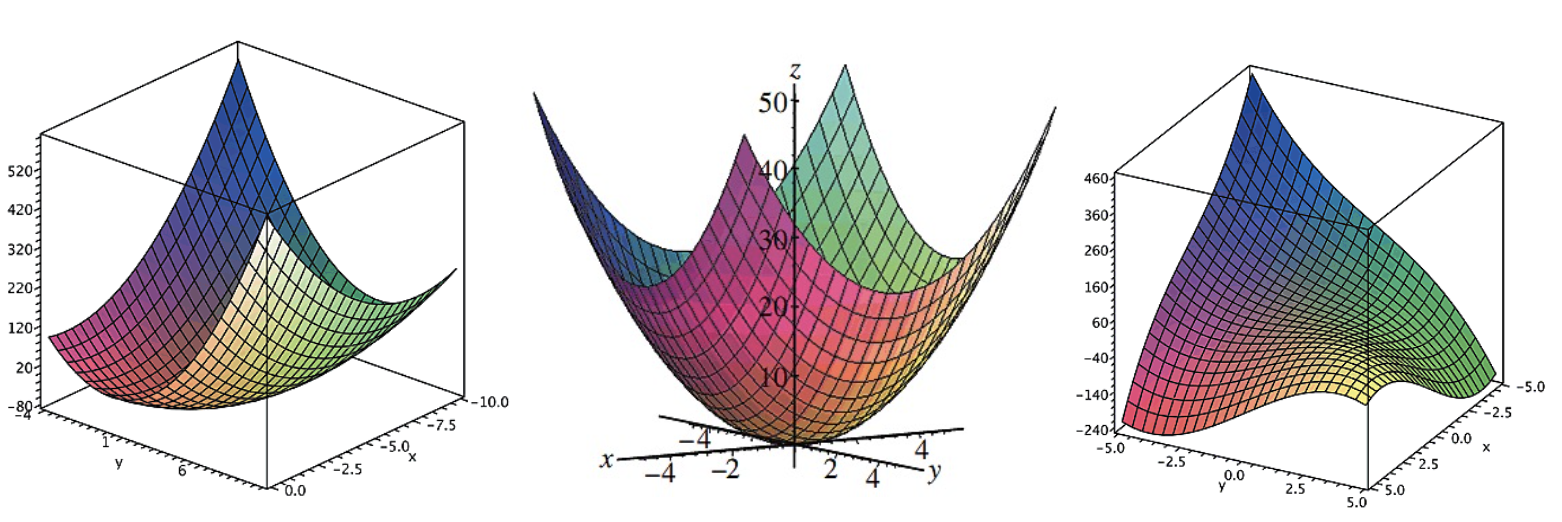
\includegraphics[width=0.5\linewidth]{./figures/F9_1.png}
  \label{fig:F9_1}
\end{figure}

\section{Indledende bemærkninger}
Hvis vi har en funktion over flere variable $f(x,y)$ kan vi integrere den ene variabel, såsom $x$, ud som
\[ 
\int_{a}^{b} f(x,y) \, \mathrm{d}x 
.\]
Her svarer det til, som var tilfældet med differentialregning i flere variable, at integrere $x$ med $y$ holdt konstant.

\begin{eks}[Simpel enkelt-integration af funktion i flere variable]
  Vi ønsker at integrere funktionen
  \[ 
  f(x,y) = x^2y^3
  ,\]
  ift. $x$. Så vi ønsker at finde
  \[ 
  \int_{0}^{1} f(x,y) \, \mathrm{d}x = \int_{0}^{1} x^2y^3 \, \mathrm{d}x 
  .\]
  Vi husker at $y$ er konstant og vi sætter derfor denne udenfor integralet
  \[ 
    y^3 \int_{0}^{1} x^2 = y^3 \left[ \frac{1}{3}x^3 \right]_0^1
  .\]
  Og vi har dermed at
  \[ 
  \int_{0}^{1} f(x,y) \, \mathrm{d}x = \frac{y^3}{3}
  .\]
\end{eks}
Vi ser fra eksemplet ovenfor at ved at vi ved at integrere $x$ ud får et udtryk der afhænger af $y$. Noget tilsvarende havde været gældende hvis vi havde integreret $y$ ud. Faktisk vil noget tilsvarende altid være gældende -- ved at integrere en variabel ud af en funktion i flere variable får du et udtryk af $n-1$ variable, hvor $n$ er antallet af variable i den oprindelige funktion.


\section{Integration over rektangler}
\begin{definition}[planintegralet]
    Lad $z = f(x,y)$ være en positiv funktion af to variable og lad $R$ betegne et rektangel
    \[ 
    a \leq x \leq b \text{og} c \leq y \leq d
    .\]
    Så har vi at 
    \[ 
    \iint_R f(x,y) \, \mathrm{d}x \, \mathrm{d}y = \int_{c}^{d} \int_{a}^{b} f(x,y) \, \mathrm{d}x \, \mathrm{d}y 
    .\]
    Dette forstås som at integrere funktionen to gange. Først integreres den ene variabel ud og dernæst integreres den anden variabel ud. Husk i øvrigt fra reglen før at hvis din funktion kun er i to variable vil planintegralet give et tal -- arealet under kurven.
\end{definition}

\begin{eks}[simpelt planintegral]
  Vi har en funktion
  \[ 
  f(x,y) = x^2y^3
  ,\]
  som skal integreres over rektanglen, $R$, defineret ved
  \[ 
  R = 0 \leq x \leq 1 \text{og} 0 \leq y \leq 2
  .\]
  Det er så at sige dette område $R$ som vi ``integrerer over''. Vi ønsker nu at udregne planintegralet af funktionen. Vi starter med at sætte afgrænsningerne ind
  \[ 
  \int_{0}^{2} \int_{0}^{1} x^2y^3 \, \mathrm{d}x \, \mathrm{d}y 
  .\]
  Først udregnes det inderste integrale givet ved
  \[ 
  \int_{0}^{1} x^2y^3 \, \mathrm{d}x 
  ,\]
  resultatet heraf er tidligere fundet til
  \[ 
  \int_{0}^{1} x^2y^3 \, \mathrm{d}x = \frac{y^3}{3}
  .\]
  Dette integreres nu over $y$-intervallet så
  \begin{align*}
    \int_{0}^{2} \frac{y^3}{3} \, \mathrm{d}y &= \frac{1}{3} \int_{0}^{2} y^3 \, \mathrm{d}y \\
    &= \frac{1}{3} \left[ \frac{y^4}{4} \right]_0^2  \\
    &= \frac{1}{3} \cdot \frac{1}{4} \cdot 2^4 \\
    &= \frac{4}{3}
  .\end{align*}
  Altså er volumenet under funktionen $x^2y^3$ i intervallet $0 \leq x \leq 1$ og $0 \leq y \leq 2$ lig 4/3.
\end{eks}

\begin{sæt}[Fubinis sætning]
  Der gælder at
  \[ 
  \int_{c}^{d} \int_{a}^{b} f(x,y) \, \mathrm{d}x \, \mathrm{d}y = \int_{a}^{b} \int_{c}^{d} f(x,y) \, \mathrm{d}y \, \mathrm{d}x 
  \]
  dvs. integrationsrækkefølgen ingen betydning har.
\end{sæt}


\section{Integration over generelle områder}
Alting bliver en smule mere kompliceret såfremt integrationsoverfladen ikke er et rektangel men et mere \emph{generelt} område. Vi har følgende definition

\begin{figure} [ht]
  \centering
  \caption{Eksempel på et type 1 og et type 2 område}
  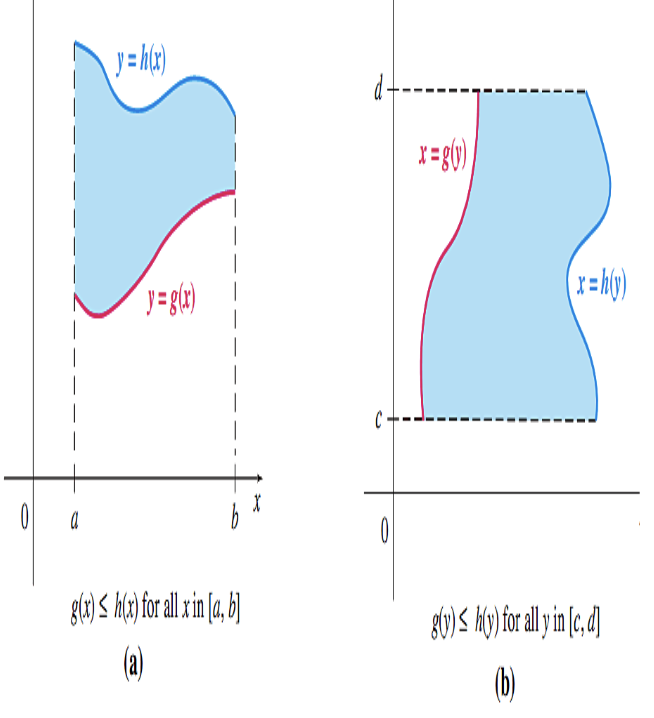
\includegraphics[width=0.4\linewidth]{./figures/F9_2.png}
  \label{fig:F9_2}
\end{figure}

\begin{definition}[Type 1 og type 2 områder]
  Vi har generelt at der eksisterer to typer af områder defineret som
  \begin{itemize}
    \item Type 1: $a \leq x \leq b$ og $g(x) \leq y \leq h(x)$
    \item Type 2: $g(y) \leq x \leq h(y)$ og $c \leq y \leq d$
  \end{itemize}
  Vi har altså for type 1 områder et overfladeintegrale på formen
  \[ 
  \iint_{R} f(x,y) \, \mathrm{d}x \, \mathrm{d}y = \int_{a}^{b} \int_{g(x)}^{h(x)} f(x,y) \, \mathrm{d}x \, \mathrm{d}y  
  .\]
  Og for type 2 områder et overfladeintegrale på formen
  \[ 
  \iint_R f(x,y) \, \mathrm{d}x \, \mathrm{d}y = \int_{g(y)}^{h(y)} \int_{c}^{d} f(x,y) \, \mathrm{d}x \, \mathrm{d}y 
  .\]
  Se evt. \autoref{fig:F9_2}.
\end{definition}

\begin{eks}[Et mere kompliceret eksempel]
  Vi ønsker at finde
  \[ 
  \iint_R \left( x^3 + 4y \right) \, \mathrm{d}y \, \mathrm{d}x 
  \]
  hvor $R$ er begrænset af
  \[ 
  y = 4x \text{og} y = x^3
  .\]
  De to funktioners skæringspunkter er i hhv. $x = 0$ og $x = 2$ og vi kan derfor tænke på det som et type 1 område og vi kan derfor opstille følgende planintegrale idet $x^3 \leq 4x$ for alle $x = [0;8]$
  \[ 
  \int_{0}^{2} \int_{x^3}^{4x} x^3 + 4y \, \mathrm{d}y \, \mathrm{d}x 
  .\]
  Vi opskriver først det inderste integral
  \[ 
    \int_{x^3}^{4x} x^3 4y \, \mathrm{d}y = [x^3y + 2y^2]_{y = x^3}^{y = 4x}
  .\]
  Vi indsætter integrationsgrænserne så vi får at
  \[
    \left( x^3 \cdot 4x + 2 \cdot (4x)^2 \right) - \left( x^3 \cdot x^3 + 2 x^{3^2} \right) = 4x^{4} + 32x^2 - 3x^{6}
  .\]
  Vi beregner nu det yderste integrale
  \begin{align*}
    \int_{0}^{2} 4x^{4} + 32x^2 - 3x^{6} \, \mathrm{d}x &= [\frac{4}{5} x^{5} + \frac{32}{3}x^3 - \frac{3}{7}x^{7}]_{x = 0}^{x = 2}  \\
    &=  56,07\ldots
  .\end{align*}
  Altså er volumenet af funktionen $f(x,y) = x^3 + 4y$ over området mellem funktionerne $y = 4x$ og $y = x^3$ lidt over 56.
\end{eks}



    \newpage
    \input{lec_10.tex}
    \newpage
    \lecture{11}{11. November 2024}{Sandsynlighedsregning 1}

\section{Stokastiske variable}
En stokastisk variabel $X$ angiver værdien af et \textit{stokastisk eksperiment}. Dette kunne eksempelvis være et terningekast. Normalt skrives stokastiske variable med store bogstaver, f.eks. $X$, $Y$ og $Z$.

For at kunne beskæftige os med forskellige typer af stokastiske variable skal vi først igennem lidt basal mængdelære.

\subsection{Tællelige mængder}
En mængde $A$ kaldes tællelig hvis vi kan skrive $A$ på formen
\[ 
  A = {a_n: \, n \in \mathbb{N}}
\]
hvor $\mathbb{N} = {1, 2, 3, \ldots}$ angiver de naturlige tal. Altså er alle mængder, hvor vi kan ``tælle'' alle elementerne ved at indicere dem \textit{tællelige}.

Det gælder generelt at alle endelige mængder er tællelige og desuden kan vises at både de naturlige tal $\mathbb{N} = {1, 2, 3, \ldots}$, de relle tal $\mathbb{Z} = {\ldots, -2, -1, 0, 1, 2, \ldots}$ og de rationelle tal $\mathbb{Q} = {\frac{a}{b}: \, a, b \in \mathbb{Z}, b \neq 0}$ samt alle deres delmængder er tællelige.

\textit{Ikke-tællelige mængder} inkluderer ethvert kontinuert interval, f.eks. $(a, b)$ eller $(a, b]$ hvor $a < b$. Altså gælder det også at de irationelle tal er ikke-tællelige og dermed er de relle tal $\mathbb{R}$ og de komplekse tal $\mathbb{C}$ begge ikke-tællelige.


\subsection{Diskrete stokastiske variable}
\begin{definition}
  En stokastisk variabel der antager værdier i en \textit{tællelig} mængde kaldes \textit{diskret}. Så alle stokastiske variable der antager værdier i endelige mængder, $\mathbb{N}$, $\mathbb{Z}$ eller $\mathbb{Q}$ er diskrete. 
\end{definition}

For at arbejde med diskrete stokastiske variable skal vi bruge summer og for de kontinuerte stokastiske variable skal vi bruge integraler. Ellers er de to typer af stokastiske variabler analoge.

\subsubsection{Sandsynlighedsfunktionen}
\begin{sæt}[sandsynlighedsfunktionen]
  Sandsynlighedsfunktionen (Eng: \textit{Probability mass function} er givet ved
  \[ 
  p(x) = P(X = x)
  .\]
\end{sæt}

Altså er sandsynligheden $p$ for at hændelsen $x$ sker lig sandsynligheden for at vores stokastiske variabel $X$ er lig vores hændelse $x$. Hvis $X$ er diskret så findes der tal $x_n$ for $n = 1,2,3,\ldots$ så at
  \[ 
  p(x_n) \geq 0
  \]
og hvor $p(x) = 0$ for alle andre værdier af $x$ ikke inkluderet i $x_n$. 

\begin{sæt}
    Idet vi ved at sandsynligheden for at vores stokastiske variabel ligger i hele området er 1 må det gælde at
  \[ 
  \sum_{n = 1}^{n} p(x_n) = 1
  .\]
\end{sæt}

\section{Middelværdi}
Givet et stokastisk eksperiment ønsker vi ofte at få nogle tal ud som vi kan fortolke. Det hyppigst brugte tal for en stokastisk model er \textit{middelværdien}.

\begin{definition}[Middelværdien]
  Hvis $X$ er en diskret stokastisk variabel med sandsynlighedfunktion $p$ så er \textit{middelværdien} $E[X]$ givet ved
  \[ 
    E[X] = \sum_{n = 1}^{n} x_n p(x_n)
  .\]
\end{definition}

Den ovenstående definition af middelværdien antager samme form som et vægtet gennemsnit af alle de værdier som vores stokastiske variabel $X$ kan antage og sandsynligheden $p(x_n)$ for at den stokastiske variabel $X$ antager værdien $x_n$. Dette er en \textit{meget vigtigt} formel.

\subsection{Gennemsnittet}
Grundet stokastiske eksperimenters grundlæggende og indbyggede tilfældighed kan vi ikke sige hvilken ``værdi'' de giver, men vi kan derimod udregne en \textit{gennemsnitsværdi} for eksperimentet, hvis vi har tilpas mange observationer. Vi kan eksempelvis ikke sige hvilken værdi et terningekast giver, men vi ved at vi i gennemsnit kan forvente at få \num{3,5}. Dette er ligeledes middelværdien idet
\[ 
  E[X] = 1 \cdot \frac{1}{6} + 2\cdot \frac{1}{6} + 3 \cdot \frac{1}{6} + 4 \cdot \frac{1}{6} + 5\cdot \frac{1}{6} + 6 \cdot \frac{1}{6} = \num{3,5} 
.\]

\begin{sæt}[Gennemsnittet konvergerer mod middelværdien]
  Mere generelt har vi at hvis $G_n = \frac{1}{n}(X_1 + X_2 + \ldots + X_n)$ angiver gennemsnittet af $n$ uafhængige og ens fordelte stokastiske variable, alle fordelt som $X$. Så vil
  \[ 
    G_n \to E[X], \quad \text{for} \quad n \to \infty
  .\]
\end{sæt}

\subsection{Fysisk fortolkning af middelværdien}
Givet en vægtløs stang, hvor vægte med massen $p(x_n)$ er placeret i punkterne $x_n$ så er middelværdien lig stangens tyngdepunkt.

\begin{eks}[Beregning af middelværdien]
  Antag 
  \[ 
  P(X = -1) = \num{0,2}, \qquad P(X = 0) = \num{0,5}, \qquad P(X = 1) = \num{0,3} 
  .\]
  Find middelværdien.
  \bigbreak
  Vi har at $x_1 = -1$, $x_2 = 0$ og $x_3 = 1$. Altså får vi at
  \[ 
    E[X] = -1 \cdot \num{0,2} + 0 \cdot 0.5 + 1 \cdot \num{0,3}  = \num{0,1}  
  .\]
  Altså er middelværdien \num{0,1}. 
\end{eks}


\section{Middelværdi af en funktion på en stokastisk variabel}
I mange sammenhænge er man interesseret i at finde middelværdien af en funktion $g$ taget på en stokastisk variabel. Eksempelvis når man skal finde variansen af stokastiske variable skal man benytte $g(X) = x^2$.

\begin{sæt}[Middelværdi af en funktion på en stokastisk variabel]
  Lad $X$ være en stokastisk variabel med sandsynlighedfunktion $p$ og lad $g$ betegne en funktion. Så har vi at
  \[ 
    E[g(X)] = \sum_{n = 1}^{n} g(x_n) p(x_n)
  .\]
\end{sæt}

\begin{eks}[Beregning af middelværdien for en funktion på en stokastisk variabel]
  Vi ønsker at finde $E[x^2]$ for tallene fra sidste eksempel så vi har altså $E[g(X)]$ med $g(X) = x^2$. Altså får vi at
  \[ 
    E[x^2] = (-1)^2 \cdot \num{0,2} + 0^2 \cdot \num{0,5} + 1^2 \cdot \num{0,3} = \num{0,5}   
  .\]
\end{eks}

Dog skal man, når man bruger ovenstående, være opmærksom på at $E[g(X)] \neq g(E[X])$. Dette ses også idet $E[x^2] = \num{0,5} \neq g(E[x]) = \num{0,1}^2$.

\begin{sæt}[Linearitet af middelværdien og momenter]
  Hvis $a$ og $b$ er konstanter så gælder at
  \[ 
    E[aX + b] = aE[X] + b
  .\]
  Hvilket er et meget nyttigt resultat. 

  \vspace{14pt} 

  \textbf{Specialtilfælde:} \hfill \\
  Hvis $k = 1,2,3, \ldots $ så kaldes $E \left[ X^k \right]$ for \textit{det $k$'te moment af $X$}. Fra det ovenstående gælder der at
  \[ 
  E \left[ X^k \right] = \sum_{n = 1}^{n} x_n^k p(x_n)
  .\]
\end{sæt}

\section{Varians}
Mens middelværdien siger noget om hvor stor den stokastiske variabel gennemsnitligt er, siger variansen noget om hvor tæt den stokastiske variabel \textit{typisk} er på sin middelværdi -- Er der stor varians kan ens resultater være sværere at stole på end hvis der er lille varians.

\begin{definition}
  Lad $X$ være en stokastisk variabel og lad $\mu = E[X]$ betegne middelværdien af $X$. Så er variansen af $X$ givet ved 
  \[ 
    \mathrm{Var}(X) = E[(X-\mu)^2]
  .\]
  Variansen er altså \textit{middelværdien} af den kvadrerede afstand mellem den stokastiske variabel $X$ og den normale middelværdi $\mu$. Det ovenstående kan også skrives som
  \[ 
    \mathrm{Var}(X) = E[X^2] - E[X]^2
  .\]
  Alstå er variansen lig 2.-momentet af $X$ minus middelværdien af $X$ i anden potens.
\end{definition}

\subsection{Fysisk fortolkning af variansen}
Mens middelværdien tidligere blev beskrevet som \textit{tyngdepunktet} af en stang kan variansen fortolkes som \textit{inertimomentet}, hvilket også kan ses af formlen. 

\begin{eks}[Variansen af et terningekast]
  Først findes 2.-momentet af den stokastiske variabel som
  \[ 
  E \left[ x^2 \right] = \frac{1}{6} \left( 1^2 + 2^2 + 3^2 + 4^2 + 5^2 + 6^2 \right) = \num{15,1666} 
  .\]
  Og vi har tidligere fundet middelværdien af et terningekast til $E[X] = \num{3,5}  \implies E[X]^2 = \num{3,5}^2 = \num{12,25}$. Altså er den samlede varians af et terningekast
  \[ 
    \mathrm{Var}(X) = \num{15,1666} - \num{12,25}  = \num{2,9166} 
  .\]
\end{eks}

Vi har fra definitionen af variansen at
\[ 
\mathrm{Var}(X) = E \left[ (X-\mu)^2 \right]
.\]
Dette er blot middelværdien af en funktion og det kan derfor skrives som
\[ 
  E \left[ (X-\mu)^2 \right] = \sum_{n = 1}^{n} (x_n - \mu)^2 p(x_n)
.\]
Og idet $(x_n - \mu)^2 \geq 0$ og $p(x_n) \geq 0$ må det gælde at $\mathrm{Var}(X) \geq 0$. Så vi har altså at
\[ 
  0 \leq \mathrm{Var}(X) = E \left[ X^2 \right] - E[X]^2 \implies E[X]^2 \leq E[X^2]
.\]
Altså har vi at 2.-momentet af $X$ altid er større end middelværdien af $X$. Faktisk er de to størrelser kun lige store for $X = \mathrm{const.}$ og derfor er der streng ulighed for alle de tilfælde vi ønsker at arbejde med her.

Desuden har vi at
\[ 
  \mathrm{Var}(aX + b) = a^2\mathrm{Var}(X)
.\]
Dette betyder at multiplikation med konstanter påvirker variansen idet disse konstanter kvadrereres mens addition med konstanter ikke påvirker variansen idet disse konstanter udgår.

\subsection{Standardafvigelsen}
Standardafvigelsen er en anden vigtig størrelse. Denne er relateret til variansen med
\[ 
  \mathrm{SD}(X) = \sqrt{\mathrm{Var}(X)}
.\]
Standardafvigelsen tager, så at sige, variansen ``tilbage til de \textit{rigtige} enheder''. 

\section{Bernoulli- og binomialfordelingen}
\begin{definition}[Bernoullifordelingen] \label{afs:forber}
  En stokastisk variabel $X$ der kun antager værdierne 0 og 1 siges at være \textit{Bernoullifordelt} med parameter $p$ hvor
  \[ 
  p = P(X=1)
  .\]
  Her vil vi ofte associere 1 med success og 0 med fiasko så Bernoullifordelinger er ofte brugt i forbindelse med binære stokastiske variable.
\end{definition}

\subsection{Binomialkoefficienten}
For $n = 1,2,\ldots $ og $i = 0,1,2,\ldots, n$ er
\[ 
  \binom{n}{i} = \frac{n!}{i!(n-1)!}
.\]
$\binom{n}{i}$ (\textit{$n$ choose $i$}) angiver antallet af delmængder med $i$ elementer i som kan udtrækkes af en mængde med $n$ elementer.

\begin{definition}[Binomialfordelingen] \label{ads:forbin}
  Lad $0 \leq p \leq 1$ og $n = 1,2,3,\ldots$. En stokastisk variabel $X$ siges da at være \textit{binomialfordelt} med parametre (n, p) (hvor $p$ kaldes sandsynlighedsparameteren og $n$ kaldes antalsparameteren) hvis $X$ har sandsynlighedsfunktion givet som
  \[ 
  p(i) = \binom{n}{i}p^{i}(1-p)^{n-i}, \quad \text{for} i = 0,1,2,\ldots ,n
  .\]
  $p$ er sandsynligheden for en success så vi har altså fået $i$ successer $n-i$ fiaskoer og $\binom{n}{i}$ er antallet af permutationer af de $i$ successer. Vi kan i øvrigt bemærke at
  \[ 
    \mathrm{Bernoulli}(p) = \mathrm{Binomial}(1,p)
  .\]
  Altså er Bernoulli-fordelingen et specialtilfælde af binomialfordelingen.
\end{definition}

\subsection{Eksperimenter der er binomialfordelte}
En binomialfordeling kan eksempelvis opstå i det vi betragter et eksperiment med kun to udfald; \textit{success} eller \textit{fiasko}. Vi antager at sandsynligheden for at få success er $p$. Hvis $X$ da angiver antallet af successer der fås ved at udføre eksperimentet $n$ gange så er $X$ binomialfordelt med parametre $(n,p)$. 

\subsection{Middelværdi og varians for binomialfordelingen}
I det følgende vil vi finde et udtryk for middelværdien og variansen af binomialfordelingen.
\begin{sæt}[Middelværdi og varians for binomialfordelingen]
  Lad $X$ være binomialfordelt med parametre $(n,p)$. Så er middelværdien
  \[
    E[X] = np
  \]
  og variansen er
  \[ 
    \mathrm{Var}(X) = np(1-p)
  .\]
  \tcblower
  Lad $k = 1,2,3,\ldots$. Vi ønsker da at finde $E \left[ X^k \right]$. Vi har at
  \[ 
    E[g(X)] = \sum_{n = 1}^{n} g(x_n) p(x_n)
  .\]
  Sættes $g(x) = X^k$ fås at
  \[ 
    E \left[ X^k \right] = \sum_{i = 0}^{n} i^{k} \binom{n}{i}p^i(1-p)^{n-i} = \sum_{i = 1}^{n} i^{k-1} \binom{n}{i}p^{i}(1-p)^{n-i}
  .\]
  Vi ønsker at finde et andet udtryk for binomialkoefficienten. Vi har at
  \[ 
  i \binom{n}{i} = i\frac{n!}{i!(n-i)!} = n\frac{(n-1)!}{(i-1)!(n-i)!} = n \binom{n-1}{i-1}
  .\]
  Vi har derfor at
  \[ 
  E \left[ X^k \right] = np \sum_{i = 1}^{n} i^{k-1} \binom{n-1}{i-1}p^{i-1}(1-p)^{n-i}
  .\]
  Vi sætter $j = i-1$ og får at
  \[ 
    E \left[ X^k \right] = np \sum_{j = 0}^{n-1} (j+1)^{k-1} \binom{n-1}{j}p^j(1-p)^{n-1-j} = npE \left[ (Y+1)^{k-1} \right]
  .\]
  Hvor $Y$ er binomialfordelt med parametre $(n-1, p)$. Vi sætter $k = 1$ og får middelværdien som
  \[ 
    E[X] = npE \left[ (Y+1)^{0} \right] = np
  .\]
  Hvis vi i stedet sætter $k = 2$ fås at
  \begin{align*}
    E \left[ X^2 \right] &= npE \left[ (y+1)^1 \right] \\
    &= npE[Y+1] \\
    &= np(1+E[Y]) \\
    &= np(1+(n-1)p) \\
    &= np + (np)^2 - np^2
  .\end{align*}

  Vi er nu klar til at finde et udtryk for variansen idet vi har at
  \[ 
    \mathrm{Var}(X) = E[X^2] - E[X]^2
  .\]
  Sættes resultaterne fra ovenfor ind fås at
  \begin{align*}
    \mathrm{Var}(X) &= np + (np)^2 - np^2 - (np)^2 \\
    &= np(1-p)
  .\end{align*}
  Altså er det vist.
\end{sæt}

\begin{eks}[Kommunikationssystemer]
  Et kommunikationssystem virker hvis mindst halvdelen af dens komponenter virker. Antag at sandsynligheden for at en komponent virker er $p$. Vi ønsker at svare på hvornår et system med 5 komponenter virker bedre end et system med 3 komponenter.
  \vspace{14pt}
  Først betragtes systemet med 5 komponenter. Vi lader $X$ betengne antallet af komponenter der virker for systemet med 5 komponenter. Vi ved da at $X$ er binomialfordelt med antalsparameter 5 og sandsynlighedsparameter $p$. Vi får da at
  \[ 
  p(virker) = p(X=3) + p(X=4) + p(X=5)
  .\]
  Idet vores stokastiske variabel $X$ antages at være binomialfordelt får vi at
  \[ 
  p(virker) = \binom{5}{3}p^3(1-p)^2 + \binom{5}{4}p^{4}(1-p)^{1} + \binom{5}{5}p^{5}(1-p)^{0} = 10p^3 (1-p)^2 + 5p^{4}(1-p) + p^{5}
  .\]
  Noget tilsvarende gøres for 3-komponent systemet så
  \begin{align*}
    p(virker) &= p(X=2) + p(X=3) \\
    &= \binom{3}{2}p^2(1-p) + \binom{3}{3}p^3(1-p)^{0} \\
    &= 3p^2(1-p) + p^3
  .\end{align*}
  Vi skal derfor afgøre for hvilke $p$ det gælder at
  \[ 
  10p^3(1-p)^2 + 5p^{4}(1-p) + p^{5} > 3p^2(1-p) + p^3
  .\]
  Man kan vise at dette gælder for $p > \frac{1}{2}$. Altså er 5-komponent systemet bedre end 3-komponent systemet, hvis sandsynligheden for at et komponent virker er mere end $\frac{1}{2}$.
\end{eks}

\section{Poissonfordelingen}
\begin{definition}[Poissonfordelingen] \label{afs:forpoi}
  Lad $\lambda > 0$. Så siges en stokastisk variabel $X$ at være \textit{poissonfordelt} med parameter $\lambda$ hvis sandsynlighedsfunktionen $p$ er givet ved
  \[ 
  p(i) = \frac{e^{-\lambda i}\lambda^{i}}{i!}
  \]
  for $i = 0,1,2,\ldots$
\end{definition}

\subsection{Eksperimenter der er Poissonfordelte}
Poissonfordelte eksperimenter opstår når vi har et meget stort antal hændelser $n$ der hver har en lille sandsynlighed $p_i$. Vi antager at alle sandsynlighederne er små og hændelserne er ``næsten'' uafhængige. Så er antallat af hændelser der indtræffer approksimativt Poissonfordelt med parameter $\lambda = p_1 + \ldots + p_n$. 

Der gælder i øvrigt at hvis $X$ er binomialfordelt med $(n,p)$, hvor $n$ er stor, $p$ er lille og $np$ er moderat. Så er $X$ approksimativt Poissonfordelt med parameter $\lambda = np$.

Mere præcist har vi at hvis $x_n$ er binomialfordelt med parametre $(n, \frac{\lambda}{n})$, $p_n$ er sandsynlighedsfunktion for $x_n$ og $p$ er sandsynlighedsfunktionen for en Poissonfordeling med parameter $\lambda$ så vil
\[ 
p_n(i) \to p(i), \quad \text{for} n \to \infty  
.\]
Altså konvergerer sandsynlighedfunktionen for en binomialfordelt stokastisk variabel med sandsynlighedsfunktionen for en Poissonfordeling for $n \to \infty$.

De typiske anvendelser af Poissonfordelingen er altså at finde
\begin{itemize}
  \item Trykfejl i en bog.
  \item Antallet af mennesker i et samfund der bliver over 100 år.
  \item Antallet af forkerte telefonnumre der ringes til i løbet af en dag.
  \item Antallet af kunder der besøger et posthus en given dag.
  \item Antallet af $\alpha$-partikler, der udsendes i en fast periode fra et radioaktivt materiale.
\end{itemize}

\begin{sæt}[Middelværdien i en Poissonfordeling]
  Lad $X$ være Poissonfordelt med parameter $\lambda$. Så er middelværdien for $X$
  \[ 
    E[X] = \lambda
  .\]
  \tcblower
  Vi benytter formlen for middelværdien idet vi, dog summer til uendeligt denne gang så vi får at
  \[ 
    E[X] = \sum_{i = 0}^{\infty} \frac{ie^{-\lambda}\lambda^{i}}{i!} = \lambda \sum_{i = 1}^{\infty} \frac{e^{-\lambda}\lambda^{i-1}}{(i-1)!}
  .\]
  Vi sætter $j = i-1$ og får at
  \[ 
    E[X] = \lambda \sum_{j = 0}^{\infty} \frac{e^{-\lambda}\lambda^{j}}{j!} = \lambda
  \]
  idet sandsynlighedsfunktionen summmer til 1 og derfor udgår. Altså er det vist
\end{sæt}

\begin{sæt}[Variansen i en Poissonfordeling]
  Det kan relativt let vises at der for en Poissonfordeling gælder at
  \[ 
    \mathrm{Var}(X) = \lambda
  .\]
\end{sæt}

Altså gælder for en Poissonfordeling at
\[ 
  E[X] = \mathrm{Var}(X) = \lambda
.\]

For Poissonfordelinger ser vi ofte, at hvis en hændelse sker tilfældigt over tid så vil hændelsen forekomme i ``klumper'' således at en række hændelser sker med relativt kort tidsmellemrum. Dette giver bl.a. anledning ti eksempelvis at overvurdere truslen fra hajangreb i perioder, hvor der kommer mange angreb -- de mange angreb skyldes ikke en øget risiko men er blot et artefakt af Poissonfordelingen.

    \newpage
    \lecture{12}{18. November 2024}{Sandsynlighedsregning 2}

\section{Andre diskrete fordelinger}
Vi har fra sidst de to fordelinger
\begin{itemize}
  \item \textbf{Binomialfordelignen}: Hvor mange ud af $n$ eksperimenter er successer givet et eksperiment der kun kan være success eller fiasko
  \item \textbf{Poissonfordelingen}: Hvis du har et fast tidsinterval, hvor mange hændelser indtræffer så indenfor dette interval
\end{itemize}
I dag vil vi bl.a. kigge på ventetidsfordelinger.

\subsection{Den geometriske fordeling} \label{afs:forgeo}
Den geometriske fordeling har sandsynlighedsparameter $0 < p < 1$ og sandsynlighedsfunktion givet ved
\[ 
P(n) = p(1-p)^{n-1}, \qquad n = 1, 2, 3, \ldots 
.\]
Funktionen ovenfor kan ses som sandsynligheden for først at få $n-1$ fiaskoer og dernæst $1$ enkelt success. Altså er der også her tale om et binært eksperiment. Den geometriske fordeling siger altså noget om hvor længe man skal vente på en success; hvad er sandsynligheden for at få $n-1$ fiaskoer efterfulgt af success?

\begin{sæt}[middelværdi og varians for geometriske fordelinger]
  Middelværdien for en geometrisk fordeling kan nemt ses til at være
  \[ 
    E[X] = \frac{1}{p}
  .\]
  Og variansen er givet ved
  \[ 
    \mathrm{Var}(X) = \frac{1-p}{p^2}
  .\]
  \tcblower
  Vi har generelt en middelværdi givet ved
  \[ 
    E[X] = \sum_{n = 1}^{\infty} n p(n)
  .\]
  Og vi får dermed
  \begin{align*}
    E[X] &= \sum_{n = 1}^{\infty} n p(1-p)^{n-1} \\ 
    &= \sum_{n = 1}^{\infty} (n-1) p(1-p)^{n-1} + \sum_{n = 1}^{\infty}  p(1-p)^{n-1}  \\
  .\end{align*}
  For $n = 1$ bliver det første led 0 og vi kan derfor starte summen fra 2 i stedet
  \begin{align*}
    E[X] &= \sum_{n = 2}^{\infty} (n-1) p(1-p)^{n-1} + \sum_{n = 1}^{\infty} p(1-p)^{n-1} \\
    &= \sum_{j = 1}^{\infty} j p(1-p)^{j} + \sum_{n = 1}^{\infty} p(1-p)^{n-1} \\
    &= (1-p) \sum_{j = 1}^{\infty} j p(1-p)^{j} + \sum_{n = 1}^{\infty} p(1-p)^{n-1}
  .\end{align*}
  Vi genkender først summen $\sum_{j = 1}^{\infty} j p(1-p)^{j}$ som middelværdien
  \begin{align*}
    \sum_{j = 1}^{\infty} jp(1-p)^{j} &= E[X] \\
  .\end{align*}
  Summen $\sum_{n = 1}^{\infty} n p (1-p)^{n-1} = 1$, da vi summer sandsynlighedsfunktionen for en geometrisk fordeling over alle udfaldene og sandsynlighdeden for hele udfaldsrummet er 1 for enhver fordeling. Vi har dermed
  \begin{align*}
    (1-p) E[x] + 1 & = E[X] (1- (1-p) = 1 \\
                   &= pE[X] = 1 \\
                   &= E[X] = \frac{1}{p}
  .\end{align*}
  Altså er middelværdien for en geometrisk fordeling
  \[ 
    E[X] = \frac{1}{p}
  .\]
  \vspace{12pt}
  Noget tilsvarende kan gøres for at vise at variansen er givet som
  \[ 
    \mathrm{Var}(X) = \frac{1-p}{p^2}
  .\]
\end{sæt}

For at vise hvordan man regner med geometriske fordelinger vil et kort eksempel i det følgende præsenteres.

\begin{eks}[Træk af kugler]
  En krukke indeholder $N$ hvide kugler og $M$ sorte kugler. Kuglerne trækkes tilfældigt, én ad gangen, indtil en sort kugle er trukket. Kuglerne lægges tilbage i krukken efter hvert træk. Vi ønsker da at finde sandsynligheden for at netop $n$ hvide kugler trækkes før vi får en sort. Idet der er tilbagelægning er eksperimentet binært og vi kan derfor regne på det med den geometriske fordeling. Hvis vi sætter $X$ til at være antallet af hvide kugler, der trækkes, før vi får en sort så ved vi at $X$ er geometrisk fordelt med parameter $p = \frac{M}{N + M}$. Vi ønsker at finde sandsynligheden for $P(X = n)$. Idet $X$ er geometrisk fordelt har vi derfor at
  \[ 
  P(X = n) = p(1-p)^{n-1}
  .\]
  Hvis vi indsætter $p$ fås
  \begin{align*}
    P(X = n) &= \frac{M}{N + M}\cdot \left( 1 - \frac{M}{N+M} \right)^{n-1} \\
    &= \frac{M}{N + M}\cdot \left( \frac{N}{N + M} \right)^{n-1} \\
    &= \frac{MN^{n-1}}{(N + M)^n} \\
  .\end{align*}
  \vspace{12pt}
  Hvis vi i stedet ønsker at finde ud af hvor mange hvide kugler vi får i middel før vi får en sort sættes blot $p = \frac{M}{N + M}$ ind i formlen for middelværdi som
  \[ 
    E[X] = \frac{N + M}{M}
  .\]
\end{eks}

\subsection{Den negative binomialfordeling} \label{afs:fornegbin}
Den negative binomialfordeling er beskrevet med en sandsynlighedsparameter, $p$ og antalsparameter, $r$, $(p,r)$. Sandsynlighedsfunktionen er givet som
\[ 
  P(X) = \binom{r-1}{n-1} p^{r}(1-p)^{n-r}, \qquad n = r, r+1, \ldots 
.\]
Denne kan fortolkes som antallet af forsøg indtil $r$ successer for et binært eksperiment. Dette kunne f.eks. være, hvis man ønsker at beregne chancen for at få $r$ plat'ter, hvis man kaster en mønt, $n$ gange. Den geometriske fordeling er altså et specialtilfælde af den negative binomialfordeling, hvor $r = 1$, hvilket også kan ses af sandsynlighedsfunktionen. Det er vigtigt at være opmærksom på at binomialfordelingen og den negative binomialfordeling er forskellige fordelinger med meget forskellige fortolkninger og brugstilfælde. 

\begin{sæt}[Middelværdi og varians for den negative binomialfordeling]
  Middelværdien for den negative binomialfordeling er givet som
  \[ 
    E[X] = \frac{r}{p}
  .\]
  Og variansen er givet ved
  \[ 
    \mathrm{Var}(X) = r\cdot \frac{1-p}{p^2}
  .\]
  Disse er altså begge lig resultaterne for den geometriske fordeling skaleret med faktoren, $r$, hvilket også givet fin logisk mening idet den geometriske fordeling angiver antallet af forsøg for 1 success og den negative binomialfordeling angiver antallet af forsøg for $r$ successer.
\end{sæt}

\section{Middelværdi for summer af stokastiske variable}
Det bør bemærkes at alt i dette afsnit både gælder diskrete og kontinuerte stokastiske variable medmindre andet er anført (kontinuerte stokastiske variable er beskrevet længere nede). Den helt centrale regel for middelværdien af summer for stokastiske variable er, at middelværdien af en sum er lig summen af middelværdierne, altså
\begin{equation} \label{eq:1}
    E[\sum_{i = 1}^{n} X_i] = \sum_{i = 1}^{n} E[X_i] 
\end{equation}

Dette vil i det følgende blive illustreret med et eksempel
\begin{eks}
  Betragt følgende stokastiske variable
  \begin{itemize}
    \item X er binomialfordelt ($5,\frac{1}{3}$)
    \item Y er Poissonfordelt ($7$)
    \item Z er geometrisk fordelt ($\frac{1}{5}$)
  \end{itemize}
  Vi ønsker da at beregne
  \[ 
    E[6X + 4Y + 7Z + 2]
  .\]
  Vha. \textbf{\autoref{eq:1}} og almindelige regneregler for middelværdier kan vi omskrive ovenstående til
  \[ 
    E[6X + 4Y + 7Z + 2] = 6\cdot E[X] + 4\cdot E[Y] + 7\cdot E[Z] + 2
  .\]
  Dermed bliver problemet noget nemmere at løse. Vi betragter først $E[X]$ som
  \[ 
    E[X] = 5\cdot \frac{1}{3} = \frac{5}{3}
  .\]
  Dernæst betragtes $E[Y]$ som
  \[ 
    E[Y] = 7
  .\]
  Og slutteligt $E[Z]$ som
  \[ 
    E[Z] = \frac{1}{\frac{1}{5}} = 5
  .\]
  Vi har dermed at
  \[ 
    E[6X + 4Y + 7Z + 2] = 6 \cdot \frac{5}{3} + 4\cdot 7 + 7 \cdot 5 + 2 = 75
  .\]
\end{eks}

\section{Egenskaber ved fordelingsfunktionen (Eng: \textit{Cumulative Distribution Function}}
Det bør, som for sidste afsnit, bemærkes at alt der bliver præsenteret i dette afsnit både gælder for diskrete og kontinuerte variable.
\begin{sæt}[Fordelingsfunktionen for en stokastisk variabel]
  Fordelingsfunktioneb, $F$, for den stokastiske variabel, $X$, er givet som
  \[ 
  F(X) = P(X \leq x), \qquad x \in \mathbb{R}
  .\]
  Fordelingsfunktionen beskriver \textit{entydigt} alle fordelinger -- dvs. både kontinuerte og diskrete stokastiske variable. Dette står i modsætning til sandsynlighedsfunktionen som kun kan bruges for diskrete stokastiske variable.

  Disse fordelingsfunktioner er rigtigt smarte, for ikke nok med at vi kan regne sandsynligheden for at den stokastiske variabel er under en bestemt værdi kan vi også regne sandsynligheden for at den stokastiske variabel er i et interval idet dette blot er differensen mellem fordelingsfunktionen til to forskellige værdier af $x$.
\end{sæt}

\section{Kontinuerte stokastiske variable}
For at kunne arbejde med kontinuerte stokastiske variable er vi nødsaget til at definere, hvad forskellen på en sådan og en diskret stokastisk variabel er. Vi arbejder med følgende definitioner
\begin{definition}[Diskrete stokastiske variable]
  En stokastisk variabel, der antager værdier i en \textit{tællelig} mængde kaldes \textit{diskret}.
\end{definition}

\begin{definition}[Kontinuerte stokastiske variable]
  En stokastisk variabel, $X$, kaldes \textit{kontinuert}, hvis der findes en positiv funktion $f$ så at for alle $A \subseteq \mathbb{R}$ vi har
  \[ 
  P(X \in A) = \int_A f(x) \, \mathrm{d}x
  .\]
  Altså, er den stokastiske variabel kontinuert, hvis man kan udregne sandsynligheden for at den stokastiske variabel $X$ ligger i en mængde $A$ ved at integrere over $A$ for alle $A \subseteq \mathbb{R}$. Funktionen $f$ for hvilken ovenstående gælder for en given stokastisk variabel kaldes tæthedsfunktionen for selvsamme stokastiske variabel.
\end{definition}

Der er desuden næsten 1:1 korrespondance mellem sandsynlighedsfunktionen for diskrete stokastiske variable og tæthedsfunktionen for kontinuerte stokastiske variable og de kan i langt de fleste tilfælde tænkes som tilsvarende koncepter, men for forskellige slags stokastiske variable.

\begin{sæt}[Punktsandsynligheder for kontunierte stokastiske variable]
  Hvis $X$ er en kontinuert stokastisk variabel så er
  \[ 
  P(X = x) = 0, \qquad \text{for alle } x
  .\]
  Dette følger fra
  \[ 
  P(X = x) = P(X \in \{ x \} ) = \int_{x}^{x} f(s) \, \mathrm{d}s = 0
  .\]
  Da $\sum_{n = 1}^{\infty} p(x_n) = 1$ for diskrete stokastiske variable kan en stokastisk variabel ikke både være kontinuert og diskret -- de to slags stokastiske variable siges at være disjunkte.
\end{sæt}

Det uegentlige integrale af tæthedsfunktionen (dvs. fra $-\infty$ til $\infty$) er
\[ 
  \int_{-\infty}^{\infty} f(x) \, \mathrm{d}x = 1
,\]
da
\[ 
  P(X \in \mathbb{R}) = 1
.\]

\begin{eks}[Ventetiden indtil en computer går i stykker]
  Lad $X$ betegne ventetiden indtil en computer går i stykker. Antag at $X$ er kontinuert med tæthedsfunktionen
  \[ 
  f(x) = \frac{1}{100}e^{-\frac{x}{100}}, \qquad 0 \leq x \text{ og } f(x) = 0 \text{ for } x<0
  .\]
  Vi ønsker da at finde sandsynligheden for at der går mellem 50 og 150 tidsenheder før computeren går i stykker. Vi ønsker altså at finde $P(50 \leq X \leq 150)$. Vi integrerer altså tæthedsfunktionen over intervallet
  \begin{align*}
    P(50 \leq X \leq 150) &= \int_{50}^{150} \frac{1}{100} e^{-\frac{x}{100}} \, \mathrm{d}x \\
    &= \left[ -e^{-\frac{x}{100}} \right]_{50}^{150} \\
    &= -e^{-\frac{3}{2}} + e^{-\frac{1}{2}} \\
    &= \num{0,38} 
.\end{align*}
\end{eks}

\subsection{Middelværdi og varians for kontinuerte stokastiske variable}
Hvor vi i ``den diskrete verden'' arbejdede meget med summer arbejder vi i ``den kontinuerte verden'' med integraler. For de diskrete variable er middelværdien \textit{summen af de værdier} den stokastiske variabel kan antage vægtet med \textit{sandsynlighedsfunktionen} medens den for de kontinuerte variable er \textit{integralet over de værdier} den stokastiske variabel kan antage vægtet med \textit{tæthesfunktionen}.

\begin{sæt}[Middelværdien for en kontinuert stokastisk variabel]
  Middelværdien for en kontinuert stokastisk variabel $X$ er givet ved
  \[ 
    E[X] = \int_{-\infty}^{\infty} xf(x) \, \mathrm{d}x 
  .\]
\end{sæt}

Vi ønsker at bruge dette i praksis og tager derfor et hurtigt eksempel

\begin{eks}[Middelværdien for en kontinuert stokastisk variabel]
  Lad $X$ have tæthedsfunktion
  \[ 
    f(x) = 2x, \text{ for } 0\leq x\leq 1 \text{ og } f(x) = 0 \text{ ellers}
  .\]
  Vi ønsker da at finde middelværdien af $X$. Af tæthedsfunktionen ses at $X$ kun antager værdier mellem 0 og 1. Hvis vi bruger formlen for middelværdien fra før får vi at
  \begin{align*}
    E[X] &= \int_{-\infty}^{\infty} xf(x) \, \mathrm{d}x  \\
    &= \int_{0}^{1} x(2x) \, \mathrm{d}x  \\
    &= 2 \int_{0}^{1} x^2 \, \mathrm{d}x  \\
    &= 2 \cdot \left[ \frac{x^3}{3} \right]_0^{1} \\
    &= \frac{2}{3}
  .\end{align*}
\end{eks}

\subsection{Middelværdi for funktioner taget på kontinuerte stokastiske variable}

\begin{sæt}
  Ønsker man at finde middelværdien for en funktion taget på en kontinuert stokastisk variabel $E[g(x)]$ skal man i stedet for at integrere $x$ op mod sin tæthedsfunktion integrere $g$ op mod sin tæthedsfunktion som
  \[ 
    E[g(x)] = \int g(x) f(x) \, \mathrm{d}x  
  .\]
\end{sæt}

Det bør desuden bemærkes at der også for kontinuerte stokastiske variable gælder relationen
\[ 
  E[aX + b] = aE[X] + b
.\]

\subsection{Variansen for kontinuerte stokastiske variable}

\begin{definition}[Variansen af en kontinuert stokastisk variabel]
  Variansen for en kontinuert stokastisk variabel er givet som
  \[ 
    \mathrm{Var}(X) = E \left[ (X - \mu)^2 \right], \qquad \mu = E[X]
  .\]
  Dette kan omskrives til
  \[ 
    \mathrm{Var}(X) = E \left[ X^2 \right] - (E[X])^2
  .\]
  Hvilket er den velkendte formel for variansen som er tilsvarende den for diskrete stokastiske variable.
\end{definition}

\begin{eks}[Variansen af en kontinuert stokastisk variabel]
  Lad $X$ have tæthedsfunktionen
  \[ 
  f(x) = 2x, \qquad \text{for } 0 < x < 1 \text{ og } f(x) = 0 \text{ ellers}
  .\]
  Vi ønsker da at finde variansen af $X$. Vi har tidligere fundet middelværdien for tæthedsfunktionen givet ovenfor. Vi mangler derfor blot at finde 2.-momentet. Vi sætter $g(x) = x^2$ og har derfor $E[g(x)]$ som løses som
  \begin{align*}
    E \left[ X^2 \right] &= \int_{0}^{1} x^2 \cdot 2x \, \mathrm{d}x  \\
    &= 2 \int_{0}^{1} x^3 \, \mathrm{d}x \\ 
    &= 2 \left[ \frac{1}{4}x^{4} \right]_0^{1} \\
    &= \frac{1}{2}
  .\end{align*}
  Vi kan dermed finde variansen som
  \[ 
    \mathrm{Var}(X) = E \left[ X^2 \right] - (E[X])^2 = \frac{1}{2} - \left( \frac{2}{3} \right)^2 = \frac{1}{18}
  .\]
\end{eks}

    \newpage
    \lecture{13}{25. November}{Sandsynlighedsregning}

\section{Den uniforme fordeling (2.3)} \label{afs:foruni}
Vi betragter et interval fra $\alpha$ til $\beta$ og vi trækker et helt tilfældigt tal mellem punkterne vil valgene være uniformfordelt.
\begin{definition} [Den uniforme fordeling]
  Lad $\alpha < \beta$. En stokastisk variabel $X$ siges at være uniformfordelt på intervalet $(\alpha; \beta)$, hvis $X$ er kontinuert med tæthed
  \[ 
  f(x) = \frac{1}{\beta - \alpha}, \quad \text{for } \alpha < x < \beta, \quad \text{og } f(x) = 0 \text{ ellers}
  .\]
  Den uniforme fordeling beskriver et helt tilfældigt valg mellem $\alpha$ og $\beta$. Den uniforme fordeling på $(0, 1)$ har tæthed $f$ givet ved $f(x) = \frac{1}{1-0} =1$ for $0 < x <1$, og $f(x) = 0$ ellers.
\end{definition}

\begin{sæt} [Fordelingsfunktionen for den uniforme fordeling]
  Fordelingsfunktionen $F$ for en uniform fordeling på $(\alpha; \beta)$ er givet ved
  \[ 
  F(x) = \frac{x-\alpha}{\beta - \alpha}, \quad \text{for} \quad \alpha \leq x \leq \beta
  .\]
  Det følger af
  \[ 
  F(x) = \int_{-\infty}^{x} f(s) \, \mathrm{d}s = \int_{\alpha}^{x} \frac{1}{\beta - \alpha} \, \mathrm{d}x = \frac{x - \alpha}{\beta - \alpha}
  .\]
\end{sæt}

\begin{sæt} [Middelværdi og Varians for en uniform fordelign]
  Middelværdien $E$ af en uniformfordelt stokastisk variabel $X$ er
  \[ 
    E[X] = \frac{\alpha + \beta}{2}
  .\]
  Dette svarer til midtpunktet af $(\alpha; \beta)$.
  \bigbreak
  Variansen $\mathrm{Var}$ af en uniformfordelt stokastisk variabel $X$ er
  \[ 
  \mathrm{Var}(X) = \frac{\beta - \alpha}{12}
  .\]
  Dette svarer til intervallængden delt med 12.
  \tcblower
  Middelværdien af en stokastisk variabel er generelt givet ved
  \[ 
    E[X] = \int_{-\infty}^{\infty} x f(x) \, \mathrm{d}x 
  .\]
  Vi kan indsætte vores tæthedsfunktion $f(x)$ som
  \begin{align*}
    E[X] &= \int_{\alpha}^{\beta} x \frac{1}{\beta - \alpha} \, \mathrm{d}x \\
    &= \frac{1}{\beta - \alpha} \int_{\alpha}^{\beta} x \\
    &= \frac{1}{\beta - \alpha} \left[ \frac{1}{2}x^2 \right]_{\alpha}^{\beta} \\
    &= \frac{1}{\beta - \alpha} \cdot \frac{1}{2} \beta^2 - \alpha^2 \\
    &= \frac{1}{\beta - \alpha} \cdot \frac{1}{2}(\beta - \alpha)(\beta + \alpha) \\
    &= \frac{\beta + \alpha}{2}
  .\end{align*}
  Altså er det vist.
\end{sæt}

\begin{eks} [Uniformfordeling]
  Lad $X$ være uniformfordelt på $(0, 10)$. Bestem $P(3 < X < 7$.
  \bigbreak
  Vi vil regne dette vha. fordelingsfunktioner. Vi har fordelingsfunktionen som
  \[ 
  F(x) = \frac{x-0}{10 - 0} = \frac{x}{10}
  .\]
  Vi kan nu finde $P(3 < X < 7)$ som tilvæskten i fordelingsfunktionen fra den nedre til den øvre grænse. Vi får altså
  \[ 
  P(3 < X < 7) = \frac{7}{10} - \frac{3}{10} = \frac{2}{5}
  .\]
  Vi kunne også have gjort dette vha. integration af tæthedsfunktionen fra nedre til øvre grænse. som
  \[ 
  \int_{0}^{10} f(x) \, \mathrm{d}x 
  .\]
\end{eks}

\section{Normalfordelingen (2.4)} \label{afs:fornor}
Normalfordelingen er en af de vigtigste og hyppigst brugte fordelinger.

\begin{definition} [Normalfordeling]
  Lad $\mu \in \mathbb{R}$ og $\sigma^2 \geq 0$. En stokastisk variabel $X$ siges at være \textit{normalfordelt} med parametre $\mu$ og $\sigma^2$, hvis $X$ har tæthedsfunktion givet ved
  \[ 
  f(x) = \frac{1}{\sqrt{2\pi}\sigma}e^{\frac{(x-\mu)^2}{2\sigma^2}} \quad \text{for alle } x
  .\]
  Hvis $\mu = 0$ og $\sigma^2 = 1$ siges $X$ endvidere at være standard-normalfordelt.
\end{definition}

\begin{sæt} [Middelværdien og variansen for normalfordelingen]
  Lad $X$ være normalfordelt med parametre $\left(\mu, \sigma^2\right)$ så gælder at
  \begin{align*}
    E[X] &= \mu \\
    \mathrm{Var}(X) &= \sigma^2
  .\end{align*}
\end{sæt}

\begin{sæt} [Fordelingsfunktionen for standard-normalfordelingen]
  Fordelingsfunktionen for standard-norrmalfordelingen skrives som
  \[ 
  \Phi(x) = \frac{1}{\sqrt{2\pi}} \int_{-\infty}^{x} e^{-\frac{s^2}{2}} \, \mathrm{d}s
  .\]
  Dette integrale kan imidlertid ikke løses analytisk og man er derfor nødt til at have gang i sin lommeregner eller finde en tabel (som \autoref{fig:F13_1}) og slå op i.
\end{sæt}

\subsection{Tabel over værdier af fordelingsfunktionen for standard-normalfordelingen}
\begin{figure} [ht]
  \centering
  \caption{Tabel over værdien af $\Phi(x)$ for forskellige $x$ for standard-normalfordelingen.}
  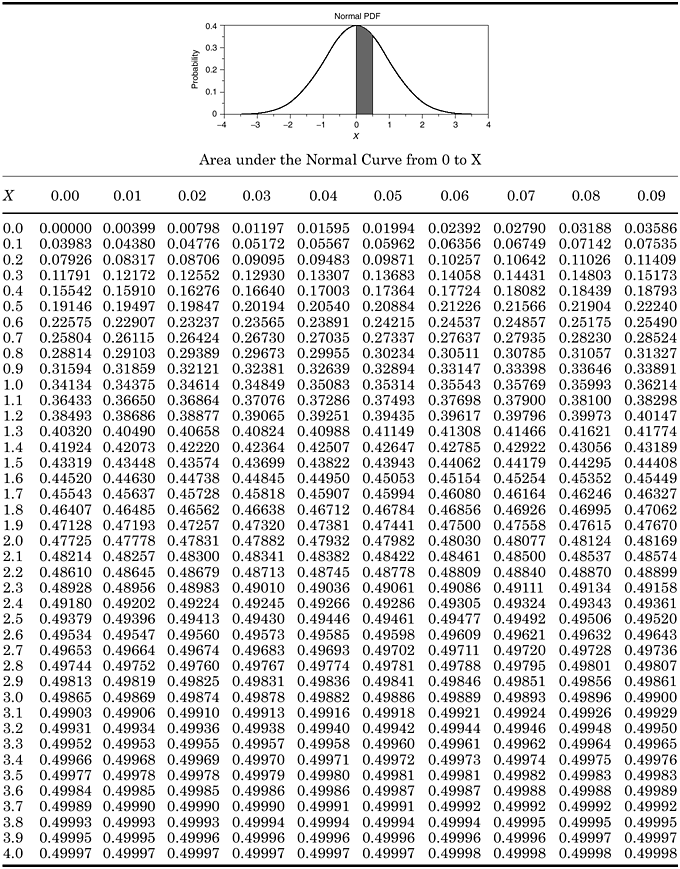
\includegraphics[width=0.8\linewidth]{./figures/F13_1.png}
  \label{fig:F13_1}
\end{figure}
Vi har desuden at $\Phi(-x) = 1 - \Phi(x)$, så hvis vi kender $\Phi(x)$ for $x > 0$ kan vi også finde $\Phi(-x)$.

Desuden gælder at hvis $X$ er normalfordelt $(\mu, \sigma^2)$ så er fordelignsfunktionen for $X$ givet ved
\[ 
F(x) = \Phi \left( \frac{x - \mu}{\sigma} \right)
.\]
Således kan man transformere en hvilken som helst normalfordeling stil standard-normalfordelingen, idet vi kan finde en generel fordelingsfunktion vha. fordelingsfunktionen for standard-normalfordelingen.

\clearpage


\subsection{Den Centrale Grænsværdi Sætning}
Normalfordelingen er en vigtig fordeling idet den er meget tæt forbundet til den centrale grænseværdi sætning. Denne er den ene af sandsynlighedsteoriens store perler, mens den anden er den såkaldte ``store tals lov'' der siger at det empiriske gennemsnit kommer vilkårligt tæt på middelværdien for store antal forsøg.

\begin{sæt} [Den Centrale Grænseværdi Sætning]
  Lad $X_1, X_2, \ldots, X_n$ være uafhængige og identiske fordelte stokastiske variable. Lad endvidere $\mu = E[X_1]$ og $\sigma^2 = \mathrm{Var}(X_1)$. Slutteligt, lad $G_n = \frac{1}{n}(X_1 + X_2 + \ldots + X_n)$ betegne deres gennemsnit. Så vil
  \[ 
  \sqrt{n}(G_n - \mu) \to Z \quad \text{for} \quad n \to \infty
  \]
  hvor $Z$ er normalfordelt med $(0, \sigma^2)$.

  Specielt vil
  \[ 
  P \left( \sqrt{n} \left( G_n - \mu\right) \leq b \right) \to \Phi\left(\frac{b}{\sigma}\right)
  \]
  Dvs. gennemsnittet er asymptotisk normalfordelt som
  \[ 
  G_n \approx N\left(\mu, \frac{\sigma^2}{n} \right)
  .\]
  \bigbreak
  Altså har ``gud'' valgt normalfordelingen som den specielle fordeling der angiver gennemsnittet af forskellige vilkårligt fordelte variable.
\end{sæt}

 Af den centrale grænseværdi sætning kan ses at normalfordelingen opstår som et resultat af en samling af mange små, tilfældige fejl eller afgivelser. 

Vi kan betragte terningekast som jo egentligt ellers er et diskret eksperiment og derfor umiddelbart ikke har meget med normalfordelingen at gøre. Vi kan dog forsøge at modellere gennemsnittet. Med en observation bliver gennemsnittet $X_1$, med to bliver det $\left( \frac{X_1 + X_2}{2} \right)$ med tre observationer er gennemsnittet $\left( \frac{X_1 + X_2 + X_3}{3} \right)$. Det her gennemsnit vil tilnærme normalfordelingen bedre og bedre for hvert kast. Dette er altså et eksempel på den centrale grænseværdi sætning.


\section{Eksponentialfordelingen} \label{afs:foreks}
\begin{definition} [Eksponentialfordelingen]
  Lad $\lambda > 0$. En stokastisk variabel $X$ siges at være \textit{eksponentialfordelt} med parameter $\lambda$, hvis $X$ har tæthedsfunktion $f$ givet ved
  \[ 
  f(x) = \lambda e^{-\lambda x}, \quad \text{for } x>0, \text{ og } f(x) = 0, \text{ ellers}
  \]
  Eksponentialfordelingen kan fortolkes til at angive ventetiden før en hændelse indtræffer, eksempelvis et jordskæv eller en krig.
\end{definition}

\begin{sæt} [Fordelingsfunktionen for eksponentialfunktionen]
  Fordelingsfunktionen $F$ er (for $x>0$)
  \[ 
  F(x) = \int_{-\infty}^{x} f(s) \, \mathrm{d}s = \int_{0}^{x} \lambda e^{-\lambda s} \, \mathrm{d}s = \left[ -e^{-\lambda s} \right]_0^{x} = 1 - e^{-\lambda x}
  \]
  For $x > 0$. Det ovenstående kan også blot skrives som
  \[ 
  F(x) = 1 - e^{-\lambda x}, \text{ fot } x>0
  .\]
\end{sæt}

\begin{sæt} [Middelværdi og varians af eksponentialfunktionen]
  Middelværdien af en eksponentialfordelt stokastisk variabel $X$ er givet ved
  \[ 
    E[X] = \frac{1}{\lambda}
  .\]
  Og variansen af en eksponentialfordelt stokastisk variabel $X$ er givet ved
  \[ 
  \mathrm{Var}(X) = \frac{1}{\lambda^2}
  .\]
  
  \tcblower
  Først udledes et udtryk for det $n$'te moment af den stokastiske variabel $X$. Vi ønsker altså at finde
  \[ 
    E\left[X^{n}\right]
  .\]
  Vi kan sætte vores tæthedsfunktion ind som
  \[ 
    E \left[ X^{n} \right] = \int_{0}^{\infty} x^{n}\lambda e^{-\lambda x} \, \mathrm{d}x 
  .\]
  Dette udtryk kan vi nu beregne vha. delvis integration som
  \begin{align*}
    \int_{0}^{b} x^{n}\lambda e^{-\lambda x} \, \mathrm{d}x &= \left[ x^{n} \left( -e^{-\lambda x} \right) \right]_0^{b} - \int_{0}^{b} n x^{n-1} \left( -e^{-\lambda x} \right) \, \mathrm{d}x \\
    &= b^{n} \left( -e^{-\lambda b} \right) - 0^{n} \left( -e^{-\lambda 0} \right) - \int_{0}^{b} nx^{n-1} \left( -e^{-\lambda x} \right) \, \mathrm{d}x  \\
    &= b^{n} \left( -e^{-\lambda b} \right) + \frac{1}{\lambda} \int_{0}^{b} nx^{n-1}\lambda e^{-\lambda x} \, \mathrm{d}x  \\
    &\implies \frac{n}{\lambda} \int_{0}^{\infty} x^{n-1}\lambda e^{-\lambda x} \, \mathrm{d}x = \frac{n}{\lambda} E[X^{n-1}]
  .\end{align*}
  Dette udtryk kan nu bruges til at beregne eksempelvis med $n = 1$ som
  \[ 
    E[X^{1}] = \frac{1}{\lambda} \cdot E[X^{0}] = \frac{1}{\lambda}
  .\]
  Vi kan gøre det samme med $n = 2$ som
  \[ 
    E[X^{2}] = \frac{2}{\lambda} \cdot E[X^{1}] = \frac{2}{\lambda^2}
  .\]
  Vi kan derfor finde udtrykket for variansen som
  \begin{align*}
    \mathrm{Var}(X) &= E \left[ X^2 \right] - E[X]^2 \\
    &= \frac{2}{\lambda^2} - \frac{1}{\lambda^2} \\
    &= \frac{1}{\lambda^2}
  .\end{align*}
  Dermed er det vist
\end{sæt}

\subsection{Fortolkning af eksponentialfordelingen}
En stokastisk variabel $X$ siges at være glemsom, hvis sandsynligheden for, at $X > t + s$, givet $X > t$, er den samme som den ubetingede sandsynlighed for, at $X > s$. Altså at sandsynligheden for, at der ikke sker f.eks. et uheld er ligeså stor for en tidsmængde $t + s$ som for en tidsmængde $t$ plus en tidsmængde $s$. 

\begin{itemize}
  \item Eksponentialfordelingen er den eneste glemsomme fordeling.
  \item Eksponentialfordelingen benyttes til at modellere ventetiden på at en hændelse sker i kontinuert tid.
  \item Eksponentialfordelingen (kontinuert) er analog til den geometriske fordeling (diskreT).
\end{itemize}

Af det ovensteånde følger, at fordelinger, hvor $X$ er glemsom er eksponential-fordelte. 



\section{Gamma fordelingen (2.6)} \label{afs:forgam}

\begin{definition} [Gamma fordelingen]
  Lad $\alpha, \lambda > 0$. En stokastisk variabel $X$ siges at være \textit{gammafordelt} med parametre $(a, \lambda)$, hvis $X$ har tæthedsfunktion $f$ givet ved
  \[ 
  f(x) = \frac{\lambda e^{-\lambda x} \left( \lambda x \right)^{\alpha-1}}{\Gamma(\alpha)}, \qquad \text{for} \qquad x > 0
  \]
  hvor $\Gamma(\alpha) = \int_{0}^{\infty} e^{-x}x^{a-1} \, \mathrm{d}x$. Igen kan $\Gamma(\alpha)$ ikke findes analytisk. Dog kan Gamma-funktionen løses i specialtilfæde, eksempelvis hvis $\lambda = 1, 2, \ldots$ er et heltal så kan integralet løses ved delvis integration hvorved løsningen bliver $(\alpha-1)!$
\end{definition}

\subsection{Fortolkning af Gammafunktionen.}
For $\alpha = 1, 2, 3, \ldots $ betegner gammafordelingen ventetiden på at $\alpha$ hændelser er indtruffet. For $\alpha = 1$ reduceres Gammafordelingen faktisk til eksponentialfordelingen
\[ 
\mathrm{eksponential}(\lambda) = \mathrm{gamma}(1, \lambda)
.\]
Hvis $X$ er $\mathrm{gamma}(\alpha, \lambda)$ så er
\begin{align*}
  E[X] &= \frac{\alpha}{\lambda} \\
  \mathrm{Var}(X) &= \frac{\alpha}{\lambda^2}
.\end{align*}
Gammafordelingen er den kontinuerte analog til den negative binomailfordeling


\section{Fordelingen af en funktion taget på stokastiske variable}
Givet
\begin{itemize}
  \item En stokastisk variabel $X$ med tæthed $f_X$.
  \item En funktion $g$.
\end{itemize}
Så ønsker vi at finde tæthedsfunktionen $f_Y$ for den stokastiske variabel $Y = g(X)$.

\subsection{Inverse funktioner}
Hvis $g$ er en kontinuert og strengt voksende/aftagende funktion, så har $g$ en \textit{invers funktion} $g^{-1}$. 

For en given $y$-værdi er $g^{-1}(y)$ det $x$ som opfylder at $g(x) = y$.

\begin{eks} [Eksempel på invers funktion]
  Vi ønsker at finde $e^{2x}$'s inverse.
  \bigbreak
  Funktionen er strengt voksende og kontinuert og har derfor en invers. Vi sætter ind som:
  \begin{align*}
    y &= g(x) \\
    y &= e^{2x} \\
    \ln(y) &= 2x \\
    x &= \frac{\ln(y)}{2}
  .\end{align*}
\end{eks}

\begin{sæt} [Transformationssætningen]
  Lad $X$ betegne en stokastisk variabel med tæthedsfunktionen $f_X$. Lad $g$ være strengt voksende/aftagende og differentiabel. Lad $g^{-1}$ betegne den inverse funktion til $g$. Lad $R = [g(x): x]$ være alle de punkter som $g$ ``rammer''. Sæt $Y = g(x)$. 

  Så har $Y$ tæthedsfunktionen $f_Y$, hvor for $y \in \mathbb{R}$
  \[ 
    f_Y(y) = f_X \left( g^{-1}(y) \right) \left| \frac{\mathrm{d}}{\mathrm{d}y} g^{-1}(y) \right|
  .\]
  og $f_Y (y) = 0$ for $y \not\in R$
\end{sæt}

\subsection{Brug af transformationssætningen}
\begin{itemize}
  \item Tjek om $g$ er strengt voksende/aftagende
  \item Find $g^{-1}$
  \item Find $\frac{\mathrm{d}}{\mathrm{d}y} g^{-1}$
  \item Find $R = {g(x): x}$
  \item Find $f_X$
  \item Indsæt i formlen:
\end{itemize}
\[ 
f_Y(y) = f_X \left( g^{-1}(y) \right) \left| \frac{\mathrm{d}}{\mathrm{d}y} g^{-1}(y) \right|
.\]

\begin{eks} [Transformationssætningen på lognormal fordelingen]
  En stokastisk variabel $Y$ siges at være lognormal fordelt, hvis $Y = e^{x}$, hvor $X$ er normalfordelt $(\mu, \sigma^2)$. Dette er en vidt-brugt model inden for bl.a. finans-verdenen idet Black-sholes-modellen kommer heraf. Vi kan benytte den ovenstående sætning  til at finde tæthedsfunktionen for en lognormal-fordelt stokastisk variabel.
  \bigbreak
  Vi sætter
  \[ 
  Y = e^{x}
  \]
  hvor $X$ er normalfordelt med $\left(\mu, \sigma^2\right)$. Dette svarer til at $g(x) = e^{x}$. Først findes den ikke-transformerede tæthedsfunktion, $f_X$ som egentligt blot er tæthedsfunktionen af normalfordelignen. Altså
  \[ 
  f_X = \frac{1}{\sqrt{2\pi}\sigma}e^{\frac{(x-\mu)^2}{2\sigma^2}}
  .\]
  Det indses hurtigt at $g$ er streng voksende og differentiabel og derfor opfylder betingelserne. 

  Vi kan nu finde $R$, som er alle punkterne som $g$ rammer. Denne rammer vilkårligt små positive reele tal og op til vilkårligt store. Altså er $R = \{g(x): x\} = \left\{ e^{x}: x \right\} = (0, \infty)$.

  Nu kan vi finde $g^{-1}$ ved at løse
  \begin{align*}
    g(x) &= y \\
    e^{x} &= y \\
    x &= \ln(y)
  .\end{align*}
  Altså er $g^{-1}(y) = \ln(y)$

  Nu kan vi differentiere $g^{-1}$ som
  \begin{align*}
    \frac{\mathrm{d}}{\mathrm{d}y} g^{-1} &= \frac{\mathrm{d}}{\mathrm{d}y} \ln(y) \\
    &= \frac{1}{y}
  .\end{align*}

  Nu kan vi indsætte i formlen idet vi husker at vores $R$ medfører at det nedenstående gælder for alle $y > 0$
  \begin{align*}
    f_Y(y) &= f_x \left( g^{-1}(y) \right) \left| \frac{\mathrm{d}}{\mathrm{d}t} g^{-1}(y) \right| \\
          &= f_X \left( \ln(y) \right) \cdot \frac{1}{y} \\
          &= \frac{1}{y}\cdot  \frac{1}{\sqrt{2\pi}\sigma}e^{\frac{(\ln(y)-\mu)^2}{2\sigma^2}}
  .\end{align*}
  Og dermed er tæthedsfunktionen for den transformerede variabel fundet.
\end{eks}

\subsection{Fordelingsfunktion vs. tæthedsfunktion: Alternativ metode til at bestemme transformerede fordelingsfunktioner}
Hvis $X$ er en stokastisk variabel med tæthedsfunktion $f$ og fordelingsfunktion $F$. Så gælder der at
\[ 
 f = F'
\]
og
\[ 
  F(x) = \int_{-\infty}^{x} f(s) \, \mathrm{d}s
.\]

Med afsæt i det ovenstående findes også en alternativ måde at bestemme $f_Y$, hvor $Y = g(X)$, idet man først kan finde fordelingsfunktionen $F_Y$ for $Y$ og dernæst finde tæthedsfunktionen $f_Y$ via $f_Y = F_Y'$.

\begin{eks} [Eksempel på brug af den alternative transformation]
  Lad $X$ være uniformfordelt på $(-1, 1)$. Vi ønsker da at finde tæthedsfunktionen for $Y = X^2$.
  \bigbreak
  Vi kan bemærke at $g(x) = x^2$ ikke er strengt voksende/aftagende ved (0,0) og derfor kan transformationssætningen ikke benyttes. I stedet kan vi benytte den alternative metode. Fordelingsfunktionen for $X$ $f_X$ er kendt idet $X$ er uniformfordelt. Vi har
  \[ 
  F_X = \frac{x - (-1)}{1 - (-1)} = \frac{x}{2} + \frac{1}{2}
  .\]
  Dette er fordelingsfunktionen for den uniforme fordeling mellem -1 og 1.

  Det første vi gør er at opskrive definitionen af fordelingsgunktionen af $Y$ som
  \[ 
  F_Y(y) = P(Y \leq y) = P \left( X^2 \leq y \right) = P \left( -\sqrt{y} \leq X \leq \sqrt{y} \right)
  .\]
  Nu har vi noget på formen $P(a \leq X \leq b)$, hvilket vi nu kan opskrive med vores fordelingsfunktion idet skarpe og bløde uligheder er ækvivalente for kontinuerte fordelinger
  \[ 
   F_Y(y) = F_X(\sqrt{y}) - F_X(-\sqrt{y})
  .\]
  Fordelingsfunktionen er kendt som $f_X = \frac{x}{2} + \frac{1}{2}$ så vi har altså
  \[ 
  F_Y(y) = \frac{\sqrt{y}}{2} + \frac{1}{2} - \left( \frac{-\sqrt{y}}{2} + \frac{1}{2} \right) = \sqrt{y}
  .\]
  Nu har vi fundet fordelignsfunktionen og tæthedsfunktionen kan derfor blot findes ved differentiation som
  \begin{align*}
  f_Y &= F_Y' \\
    &= \frac{1}{2 \sqrt{y}}
  .\end{align*}
\end{eks}

    % end lectures
\end{document}
